\documentclass[twoside,english]{uiofysmaster}

\usepackage{float}	% figurer der man plasserer dem
%\usepackage{caption}
\usepackage{verbatim}	% \begin{comment}
\usepackage{subcaption}
%\usepackage{siunitx}



%\bibliography{references}

\author{John-Anders Stende}
\title{Neural networks in molecular dynamics}
\date{May 2017}

\begin{document}

\maketitle

\begin{abstract}
This is an abstract text.
\end{abstract}

\begin{dedication}
  To someone
  \\\vspace{12pt}
  This is a dedication to my cat.
\end{dedication}

\begin{acknowledgements}
  I acknowledge my acknowledgements.
\end{acknowledgements}

\tableofcontents

\chapter{Introduction}
***Motivate the reader, outline structure of report and what we have done***

\section{Goals}
The main goal of this thesis is to use artificial neural networks to
construct many-body potential energy surfaces (PES) to be used in molecular dyanmics (MD) simulations.  
This goal can be split into the following intermediate objecives:
\begin{itemize}
 \item Train an one-dimensional ANN with the machine learning library TensorFlow (TF) 
 to reproduce the shifted Lennard-Jones (LJ) potential.
 As a first test case, we will train the NN on random data and investigate
 how different NN architectures and activation functions influence the quality of the potential fit. 
 \item Train a many-body NN to reproduce the Stillinger-Weber (SW) potential for Si. 
 Training data (configurations of particles and energies) will be sampled from SW LAMMPS simulations. 
 The resulting NNP will then be used to simulate Si with LAMMPS. 
 We therefor need to extend the LAMMPS library with our own neural network potential.
 \item Construct a many-body NNP that will be able to simulate a system consisting of several atom types. 
 The method will be tested on the Vashishta potential for SiO2.
\end{itemize}


\chapter{Theory}
***Theory needed to understand the results and implementations***

\section{Molecular dynamics}
Molecular dynamics (MD) is a method to simulate the physical movements of atoms and molecules in gases, liquids and solids. 
It is thus a type of N-body simulation. The atoms are modelled as point-like particles with interactions described
by classical force fields. Their time-evolution is governed by Newton's equations of motion. MD allows one to study the microscopic
movement of thousands or millions of atoms, enabling the sampling of macroscopic properties such at temperature, pressure, 
diffusion, heat capacity and so on. 

The dynamics of an ensemble of particles is governed by their interactions. 
In classical MD, the interactions are described
by a classical force field $\vec{F}$, which is defined as the negative gradient of a potential energy surface (PES) $E$,
\begin{equation}
 \vec{F} = -\nabla E
\end{equation}
The PES is represented by a mathematical function, often split into a sum over two- and three-body interactions. 
Instead of using an analytical functional form to represent the energy, one can 
calculate the energies and forces for each time step in the MD simulation using an ab inito method. 
Different quantum mechanical methods like Hartree-Fock (HF) and Density Functional Theory (DFT) are used for this purpose. 
These approahces to MD are called quantum-classical molecular dynamics (QCMD). 

\subsection{Potential energy surfaces}
The dynamics of an ensemble of particles is governed by their interactions. 
In classical MD, the interactions are described
by a classical force field $\vec{F}$, which is defined as the negative gradient of a potential energy surface (PES) $E$,
\begin{equation}
 \vec{F} = -\nabla E
 \label{forcePES}
\end{equation}
The expression for $V(r)$ may be obtained in different ways:
\begin{itemize}
 \item Empirical potentials: the functional form are chosen and the parameters fitted from 
 empirical knowledge about the system
 \item Semi-empirical potentials: based on methods from computational QM, but many approximations
 are made and some parameters are obatained from empirical data
 \item Quantum mechanical potentials: a computational QM method 
 is used to obtain the energy for different configurations, and then fitted by a functional form
\end{itemize}
Instead of using a pre-defined functional form to represent the energy, one can 
calculate the energies and forces for each time step in the MD simulation using an ab inito method. 
Different quantum mechanical methods like Hartree-Fock (HF) and Density Functional Theory (DFT) are used for this purpose. 
These approahces to MD are called quantum-classical molecular dynamics (QCMD). 

The PES represents the potential energy $V(\vec{r})$ of a system as a mathematical function of the configuration of the atomic 
positions $\vec{r} = (\vec{r}_1, \vec{r}_2, \dots \vec{r}_N)$. To reduce
the $N$-body problem from a fully quantum description to a classical potential we must make the Born-Oppenheimer 
approximation, which is the assumption that the motion of atomic nuclei and electrons in a molecule
can be seperated. This enables us to freeze the degrees of freedom of the nuclei and solve the electronic
Schrödinger equation with the positions of the nuclei as parameters. Varying the positions of the nuclei
in small steps and repeatedly soving the Schrödinger equation, the quantum PES is made. 
Classically, we can now approximate the atomic nuclei as point-particles that follow
Newtonian dynamics, while the positions and velocities of the electrons are baked into the PES, usually
representing the ground state. (HA ET EGET AVNSITT OM BORN-OPPENHEIMER I KVANTETEORIDELEN KANSKJE?)

As mentioned above, we represent the PES by a pre-defined functional form in classical MD. We can assume that this
function can be written as a sum of $n$-body terms,
\begin{equation}
 V(\vec{r}) \approx \sum_{i=1}^N V_1(\vec{r}_i) + \sum_{i<j}^N V_2(\vec{r}_i, \vec{r}_j) + 
 \sum_{i<j<k}^N V_3(\vec{r}_i, \vec{r}_j, \vec{r}_k) + \dots
\end{equation}
Each term can be determined by performing an electronic structure calculation for a number of configurations, 
and fitted by a suitable functional form. Determining how many terms that is sufficient to 
describe a system adequately is however not trivial. Noble gases like argon have weak interactions and 
may be well described by a two-body potential $V_2$, while molecules with strong angular dependencies on their bond, like
silicon (Si), will need at least three-body potentials $V_3$. Another challenge is to identify the
configuration space of the system. For three-body potentials and more the set of probable configurations is large, and 
running an \textit{ab inito} simulation for each configuration is expensive. This problem will be discussed below. 

An important step is how to fit the above potential terms obtained from QM calculations to a functional form. 
There exist a lot of different interpolation teqhniques; in this theses we will use ANNs to fit the data. 
(SKRIVE OM ANDRE INTERPOLASJONSTEKNIKKER?)


\subsection{LAMMPS}
(HAVE TO REFER TO THE MANUAL HERE OR SOMETHING.
DOES THAT COUNT AS AN ORDINARY REFERENCE, 
OR SHOULD IT BE A FOOTNOTE?)
LAMMPS (Large-scale Atomic/Molecular Massively Parallel Simulator)
is a classical molecular dynamics simulation package 
developed at Sandia National Laboratories. It is written
in highly portable and extendable objected-oriented c++. 
The package's functionality encompasses a wide variety of 
potentials, atom types, integrators, thermostats and 
ensembles and are able to simulate a large number
of different systems, including atoms, molecules, 
coarse-grained particles, polymers, graunular materials
and metals. LAMMPS can be run on a single processor
or in parallell. 
There exist several other molecular dynamics packages, 
like GROMACS, OpenMD, Aber and NAMD that could also
have served the purpose of this thesis. We have chosen
to work with LAMMPS because it is well documented, 
easy to expand upon and because the Computational
physics group at UiO has a lot of experience with using
it for molecular dynamics simulations. 
In this section we will outline the basic usage of LAMMPS, including
a walkthrough of an example input script. We also describe its
class hierarchy and how we can add our own functionality
to the package.

\subsubsection{Installing LAMMPS}
We have chosen to install LAMMPS by cloning
the Github repository (LINK) and compile the source
code by running $make$ in the source directory. 
To compile a serial version of the software, we simply run
the command
\begin{lstlisting}
 make serial
\end{lstlisting}
while the corresponding command for the parallel
MPI version is
\begin{lstlisting}
 make mpi
\end{lstlisting}
New updates can be downloaded by setting an
upstream git remote to point to the LAMMPS
GitHub repository and doing a $git pull upstream master$.
(TROR IKKE DETTE ER HELT RIKTIG). 
LAMMPS also have several additional packages that
can be installed. This can be done by running
\begin{lstlisting}
 make yes-<package name>
\end{lstlisting}
e.g. $manybody$ to install many-body potentials
like Stillinger-Weber and Vashishta. 

\subsubsection{LAMMPS input script}
LAMMPS is run by providing an input script as 
argument to the excecutable. This input script
is read line by line and has its own syntax. 
A good way to show the basics an input file
is to look at a simple example of a script
to measure diffusion in liquid argon 
(CHANGE LC VALUE LATER):
\begin{lstlisting}
### initialization ###
units 		metal		
dimension 	3
boundary	p p p		
atom_style	atomic		

### create geometry and atoms ###
lattice 	fcc 1.08506
variable	Nc equal 10
region 		myRegion block 0 ${Nc} 0 ${Nc} 0 ${Nc}
create_box	1 myRegion
create_atoms	1 box

### set mass and initial temperature ###
mass		1 1.0
variable	temp equal 300
velocity	all create ${temp} 87287 mom yes 

### compute diffusion ###
compute 	displacement all displace/atom

### potential ###
pair_style	lj/cut 2.5
pair_coeff	1 1 1.0 1.0 2.5
neighbor	0.5 bin
neigh_modify	every 20 delay 0 check no

### integration ###
timestep 	0.01
run_		style verlet
fix 		integration all nve

### output ###
thermo		50
thermo_style custom step temp density press ke pe etotal 
thermo_modify norm yes

### run simulation ###
run		5000
dump diffusion all custom 100 diffusion*.dat c_displacement[4]
run_		10000
\end{lstlisting}
We will in the following briefly explain what
processes that are evoked in LAMMPS when the 
above commands are read. 
\begin{lstlisting}
 units metal
\end{lstlisting}
This command defines the units that are used 
in the simulation and the output. LAMMPS have eight
different unit sets. The \textit{metal} set measures
distance in Ångstrøm, energy in eV and temperature
in Kelvin. The choice of units depend on the system
that is investigated and the scale we are looking at.
\begin{lstlisting}
 boundary p p p
\end{lstlisting}
We want to measure diffusion in a bulk
Argon liquid, thus we want to have periodic 
boundary conditions in all three dimensions, 
annotated by a $p$. LAMMPS can also handle stiff ($f$)
and adaptive ($s$) non-periodic boundaries. Adaptive
means that the position of the face is set so as to
encompass the atoms in that dimension. 
\begin{lstlisting}
 atom_style atomic
\end{lstlisting}
Different systems need different information
to be stored for each atom. For style $atomic$, only
the default attributes are associated with each atom, 
namely coordinates, velocities, atom IDs and types. 
This is sufficient for pair-interacting, non-bonded
systems like Argon.
\begin{lstlisting}
lattice 	fcc 5.720
\end{lstlisting}
Next, we set the initial configuration of the atoms. 
Here, a ffc lattice with a lattice constant of
5.720 is used. Other types of lattices based on
cubic or squared unit cells are also available. 
\begin{lstlisting}
variable	Nc equal 10
region 		simBox block 0 ${Nc} 0 ${Nc} 0 ${Nc}
\end{lstlisting}
The system's geometry is defined with the $region$
command. The $block$ style is simply a 3-dimensional
straight-faced box with a size of $N_c = 10$ unit
cells in each dimension. We have labelled the 
region $simBox$. 
The number of unit cells
$N_c$ is defined as a LAMMPS $variable$. Variables
can be referenced elsewhere in the script by
writing $\${variable}$ to become part of a new input
command like above. LAMMPS enables many styles
of variables to be defined. 
\begin{lstlisting}
create_box	1 simBox
create_atoms	1 box
\end{lstlisting}
The command $create_box$ creates a simulation box 
based on the specified region, in our case the 
$block$ region defined above. The argument specifies
the number of atom types that will be used in the
simulation. Next, $create_atoms$ with the argument
$box$ fills the simulation
domain with atoms of type 1 on the lattice. 
LAMMPS also lets you create a random collection
of atoms or single atoms at specified coordinates.
\begin{lstlisting}
mass		1 28
variable	temp equal 300
velocity	all create ${temp} 87287 
\end{lstlisting}
We need to assign mass to the atoms. For metal units, 
mass is measured in grams/mole. The atoms are also
given an initial velocity that corresponds to 
the given initial temperature. 
\begin{lstlisting}
### potential ###
pair_style	lj/cut 2.5
pair_coeff	1 1 1.0 1.0 2.5
\end{lstlisting}
The choice of potential is made with the 
$pair_style$ command. We want to simulate
interactions using the cutoff Lennard-Jones potential
with a global cutoff of 2.5 Å. The LJ parameters
are set with $pair_coeff$, the way this is done
depends on the potential being used. For our
choice of potential the arguments is as follows:
$atom-type-1 atom-type-2 sigma epsilon cutoff$. 
The parameters and cutoff can thus be set seperately 
for each pair of atom types.
\begin{lstlisting}
neighbor	0.5 bin
neigh_modify	every 20 check yes
\end{lstlisting}
These commands sets parameters that affect the 
building of neighbor lists. The first argument
to $neighbor$ is the skin size, while the 
second selects what algorithm is used
to build the lists. The $bin$ style creates 
the lists by binning, which in most cases
(including ours) is the fastest method. 
Further, we can control how often the lists
are built with $neigh_modify$. The above arguments
specifies that new neighbour lists are built 
every 20 steps, but every step LAMMPS checks
if any atom has moved more than half the skin distance.
If that is the case, new lists are built. 
\begin{lstlisting}
timestep 	0.01
run_style 	verlet
fix 		integration all nve
\end{lstlisting}
LAMMPS integrates Newtons' equations of motion
with the velocity-Verlet algorithm by defualt. 
This is the integrator of choice for most MD
applications due to its simplicity and 
symplectic nature (REF TO SECTION). The 
rRESPA integrator \cite{ref11} scheme is also available.
LAMMPS does however not integrate and update
the positions and velocities of the particles
if not explicitly told so. This is done with
a $fix$, which is any operation that is applied to the 
system during timestepping. The above fix 
tells LAMMPS to integrate all atoms in the system 
so that they follow trajectories consistent with 
the microcanonical ensemble. 
\begin{lstlisting}
thermo		50
thermo_style custom step temp press ke pe etotal 
thermo_modify norm yes
\end{lstlisting}
We can control what thermodynamic properties 
to calculate and output with $thermo_style$, while 
$thermo$ decides how often they should be computed. 
We want to output the time step, temperature, 
pressure, kinetic energy, potential energy and total
energy. Also, we want to normalize the extensive
quantities (the energies) by the number of atoms. 
\begin{lstlisting}
 compute displacement all displace/atom
 dump diffusion all custom 100 diffusion*.dat c_displacement[4]
\end{lstlisting}
To measure diffusion in the 
Argon liquid, we need to calculate the net
displacement of all atoms. This can be done with a 
$compute$, which defines a computation that is 
performed on a group of atoms, in this case all atoms.
The $displace/atom$ compute calculates the current
displacement of each atom from its original
coordinates, including all effects due to atoms
passing through periodic boundaries.
For the compute to actually be performed, it needs
to be evoked by other LAMMPS commands, like $dump$, 
which writes a snapshot of atom quantities to one 
or more files every N timesteps. Computes are 
referenced via the following notation $c_ID$, where
ID is the ID of the compute. 
\begin{lstlisting}
run		5000
\end{lstlisting}
Lastly, we run the simulation for 5000 timesteps. 
LAMMPS allowes several run commands to be issued
after one another. This comes in handy if we want
to thermalize the system before measuring diffusion.
This can be achieved by writing the following commands:
\begin{lstlisting}
 run 5000
 dump diffusion all custom 100 diffusion*.dat c_displacement[4]
 run 10000
\end{lstlisting}
When parsing the second run command, LAMMPS will
continue the dynamics while computing eventual
new fixes, computes, dumps etc. defined since
the last run command. 

This section has illuminated some of the basic
funcionality of LAMMPS through several comments
on a simple input script. Now we move on to
how class hierarchy of LAMMPS is structured. 

\subsubsection{LAMMPS structure}
LAMMPS is written in C++ in an object-oriented
fashion. The class hierarchy is shown schematically
in figure (MAKE MY OWN FIGURE IN INKSCAPE). 
The blue classes are the core classes, these
are visible anywhere in LAMMPS.
Most of these have subclasses, of which the red ones
are called style classes. We recognize many 
of the input script commands among the style
classes; a rule of thumb is that every input script
command has a corresponding class and a
corresponding file name in the source directory. 
For instance, the cutoff Lennard-Jones potential
used in our input script is a subclass of Pair,
and is evoked by the command
$pair_style lj/cut$ and the source file is named
\textit{pair_lj_cut.cpp}. 

We will not go into detail about the functionality
and communication of these classes. The class
that is the most relevant for this work is the Pair class, 
as we have implemented our own NN potential pair_style. 
In the following section we will describe how 
LAMMPS can be extended with a new pair potential
through example. 

\subsubsection{Extending LAMMPS}
To extend LAMMPS with a new potential, we 
simply add a new *.cpp and *.h file to the 
source directory and re-compile. The new class
will (in theory) work with all other LAMMPS 
classes without breaking any functionality. 
A good strategy is to start with an existing potential
source file that is somewhat similar to the one 
we want to make, instead of programming from scratch.
We aim to construct a many-body potential, and 
have chosen to base our implementation on the 
Stillinger-Weber potential file, pair_sw.cpp and -.h.



 

















\section{Machine learning}
Machine learning is the science of giving computers the ability to learn without being explicitly programmed. 
The idea is that there exist generic algorithms which can be used to find patterns in a broad class of data sets without 
having to write code specifically for each problem. The algorithm will build its own logic based on the data. 

There are two main machine learning methods, supervised learning and unsupervised learning. For the former method, 
you know the answer to a problem and let the computer deduce the logic behind it. When doing the latter, you do not
know the answer and are just trying to find patterns and relationship in the data. 

Another way to categorize machine learning tasks is to consider the desired output of a system.
Some of the most common tasks are:
\begin{itemize}
 \item Classification: Outputs are divided into two or more classes. The goal is to 
 produce a model that assigns inputs into one of these classes. An example is to identify
 digits based on pictures of hand-written ones. Typically supervised. 
 \item Regression: Find a functional relationship between variables, the outputs are thus continous. 
 \item Clustering: Inputs are divided into groups without knowing the different groups, i.e. a form of unsupervised classification.  
\end{itemize}
In this thesis we will use machine learning to do regression, i.e. to find the PES of interacting molecules.
One approach to machine learning regression is artificial neural networks. 

\section{Artificial Neural Networks}
An Artificial Neural Network (ANN) consists of layers of connected nodes, or neurons. 
It is supposed to mimic a biological nervous system by letting each neuron interact with other neurons
by sending signals between layers. The accumulated signals received by a neuron is used as input to its 
\textit{activation function}, which is used to to send new signals to following layers. This function is supposed to mimic that 
a biological neuron is activated if the input is above a certain threshold. We will here follow 
Behler \cite{ref1} and Dragly \cite{ref2}.

There are many types of ANNs made for different purposes. The most widely used are feed-forward and recurrent ANNs. 
The feedforward network was the first and arguably the most simple type of ANN. In this network the information or signals
only move forward through the layers - from the input layer, through each successive hidden layer and finally to the output layer. 
On the other hand, recurrent networks have cycles and loops, i.e. bi-directional data flow. Feed-forward neural networks, 
also called Multilayer Perceptrons (MLP) were shown to be universal function approximators by K. Hornik et al. \cite{ref3} in 1989.
We will use these networks to approximate the PES in thesis. 
\begin{figure}[H]
\begin{center}
  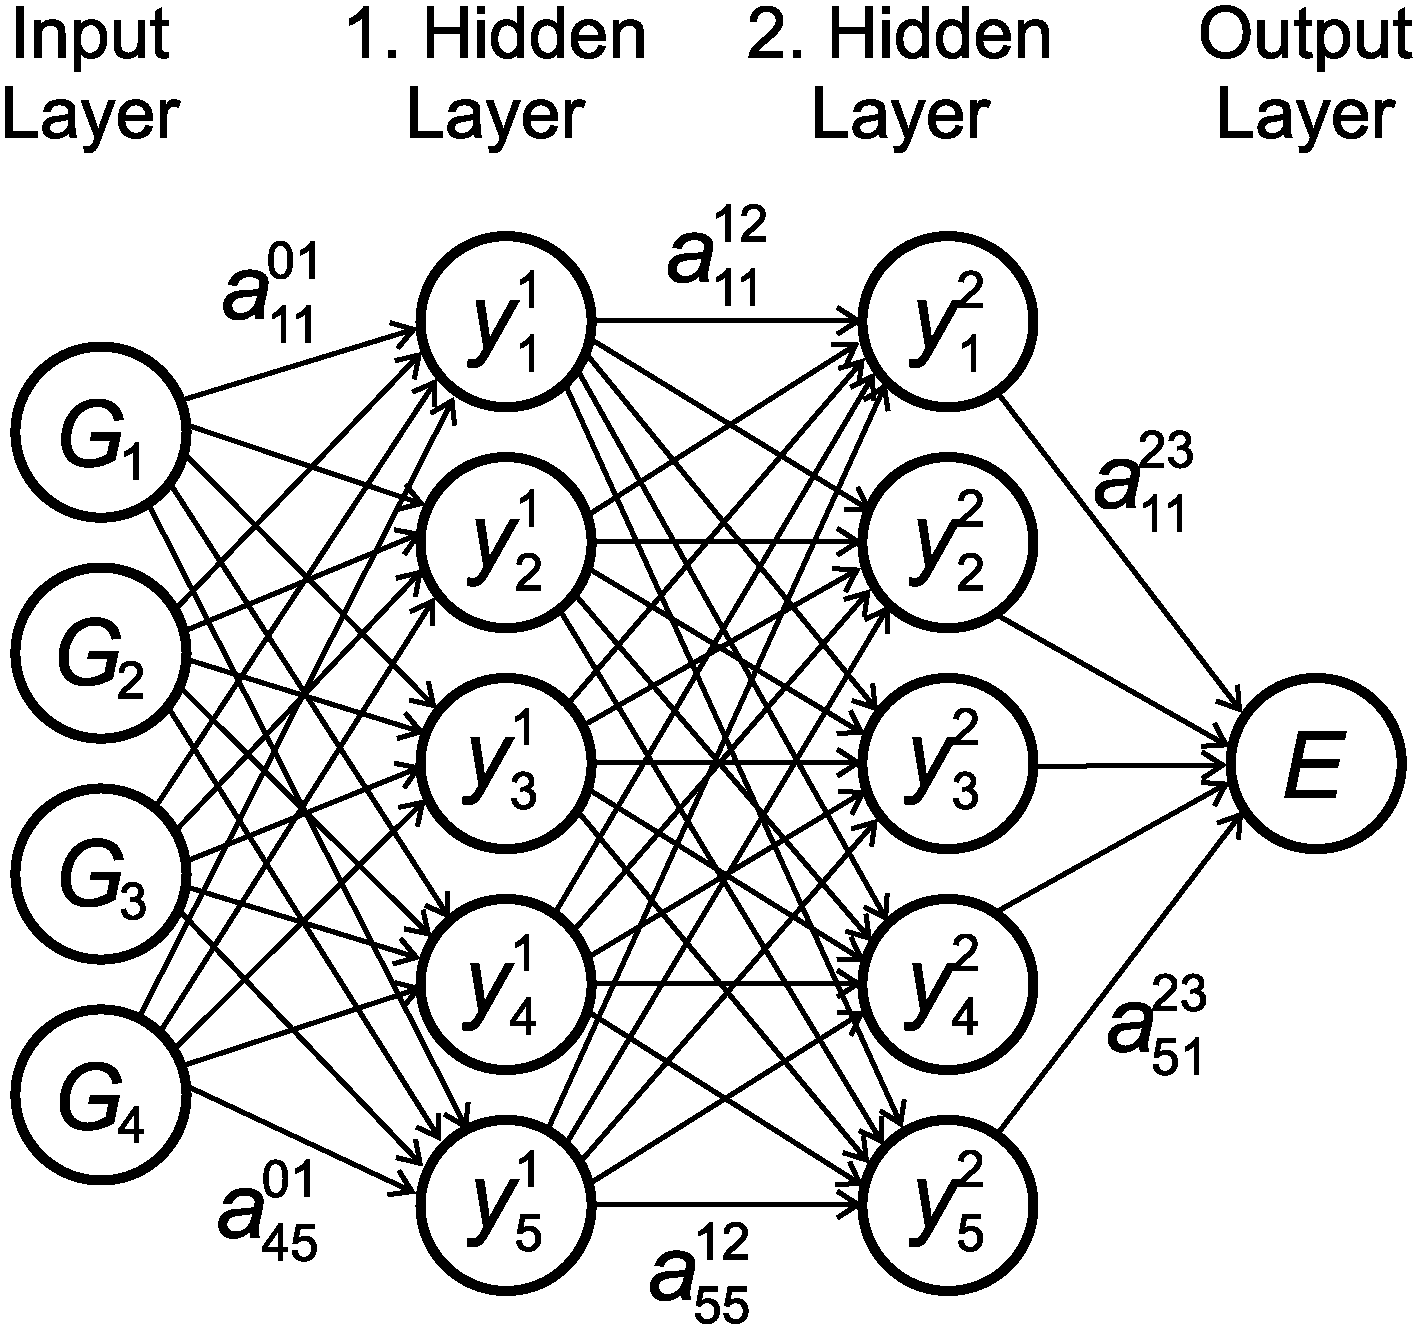
\includegraphics[width = 0.7\linewidth]{Figures/Theory/MLP.png}
  \caption{Neural network}
  \label{fig:NN}
  \end{center}
\end{figure}
An MLP networks is shown schematically in \autoref{fig:NN} (STOLEN FROM \cite{ref3}, EDIT TO ONE INPUT LATER). 

This network maps input coordinates $G_i$ to a potential energy in the output layer via two hidden layers
with an (arbitrary) number of hidden nodes. The hidden neurons have no physical meaning, but have the purpose
of defining the functional form of the NN. All nodes in each layer are connected to the nodes in the adjacent layer by
\textit{weights}, the fitting parameters of the NN. These are called fully connected layers. We use the notation
$a_{ij}^{kl}$ for the weight connecting node number $i$ in layer $k$ with node number $k$ in layer $l=k+1$. 
Also, each node in the hidden layers and the output node have a \textit{bias} $b_i^j$, where $i$ indicates
node number and $j$ layer. All weights and biases are real-valued numbers.

The output of this MLP is calculated in the following way. The configuration are specifiec by the input nodes.
Then, a weighted sum $x_m^1$ of the input coordinates ${G_i}$ is calculated for each node $m$ in the first hidden layer 1
\begin{equation}
 x_m^i = \sum_{i=1}^4 G_i a_{i,m}^{01} + b_m^i 
\end{equation}
where we also add the bias $b_m^i$ for each node. This is a linear combination of the input coordinates
using the connection weights as coordinates, which is used as input to the activation function $f_m^1$ of each neuron, thus
producing the output $y_m^1$ of all neurons in layer 1:
\begin{equation}
 y_m^1 = f_m^1(x_m^1)
\end{equation}
For an arbitrary node $m$ in a hidden layer $n$ this generalizes to
\begin{equation}
 y_m^n = f_m^n(x_m^n) = f_m^n\left(\sum_{i=1}^{N_{n-1}} y_i^{n-1}a_{i,m}^{n-1,n}\right)
\end{equation}
where $N_n$ is the number of nodes in layer $n$. When the output of all the nodes in the first hidden layer are computed,
the values of the subsequent layer can be calculated and so forth until the output is obtained. The complete functional form
of an MPL with $n$ hidden layers is thus
\begin{equation}
 E = f_1^{n+1}\biggr(\sum_m^{N_n}f_m^{n}\biggr(\sum_l^{N_{n-1}}f_l^{n-1}\biggr( \cdots \sum_j^{N_1} 
     f_j^1\biggr(\sum_{i=1}a_{i,j}^{0,1}G_i + b_j^1\biggr) \cdots \biggr)\biggr)\biggr)
     \label{completeNN}
\end{equation}
i.e. a nested sum of activation functions. A desired property of activation functions is to converge asymptotically
to constant output values for large and small arguments, with a non-linear region in-between. The non-linearity enables
the ANN to fit arbitrary functions \cite{ref3}. Common activation functions \cite{ref4} for 
function approximation are the sigmoid function
\begin{equation}
 f(x) = \frac{1}{1 + e^{-x}}
 \label{sigmoidActivationFunction}
\end{equation}
and the hyperbolic tangent
\begin{equation}
 f(x) = \tanh(x)
 \label{tanhActivationFunction}
\end{equation}
\begin{figure}[H]
\begin{center}
  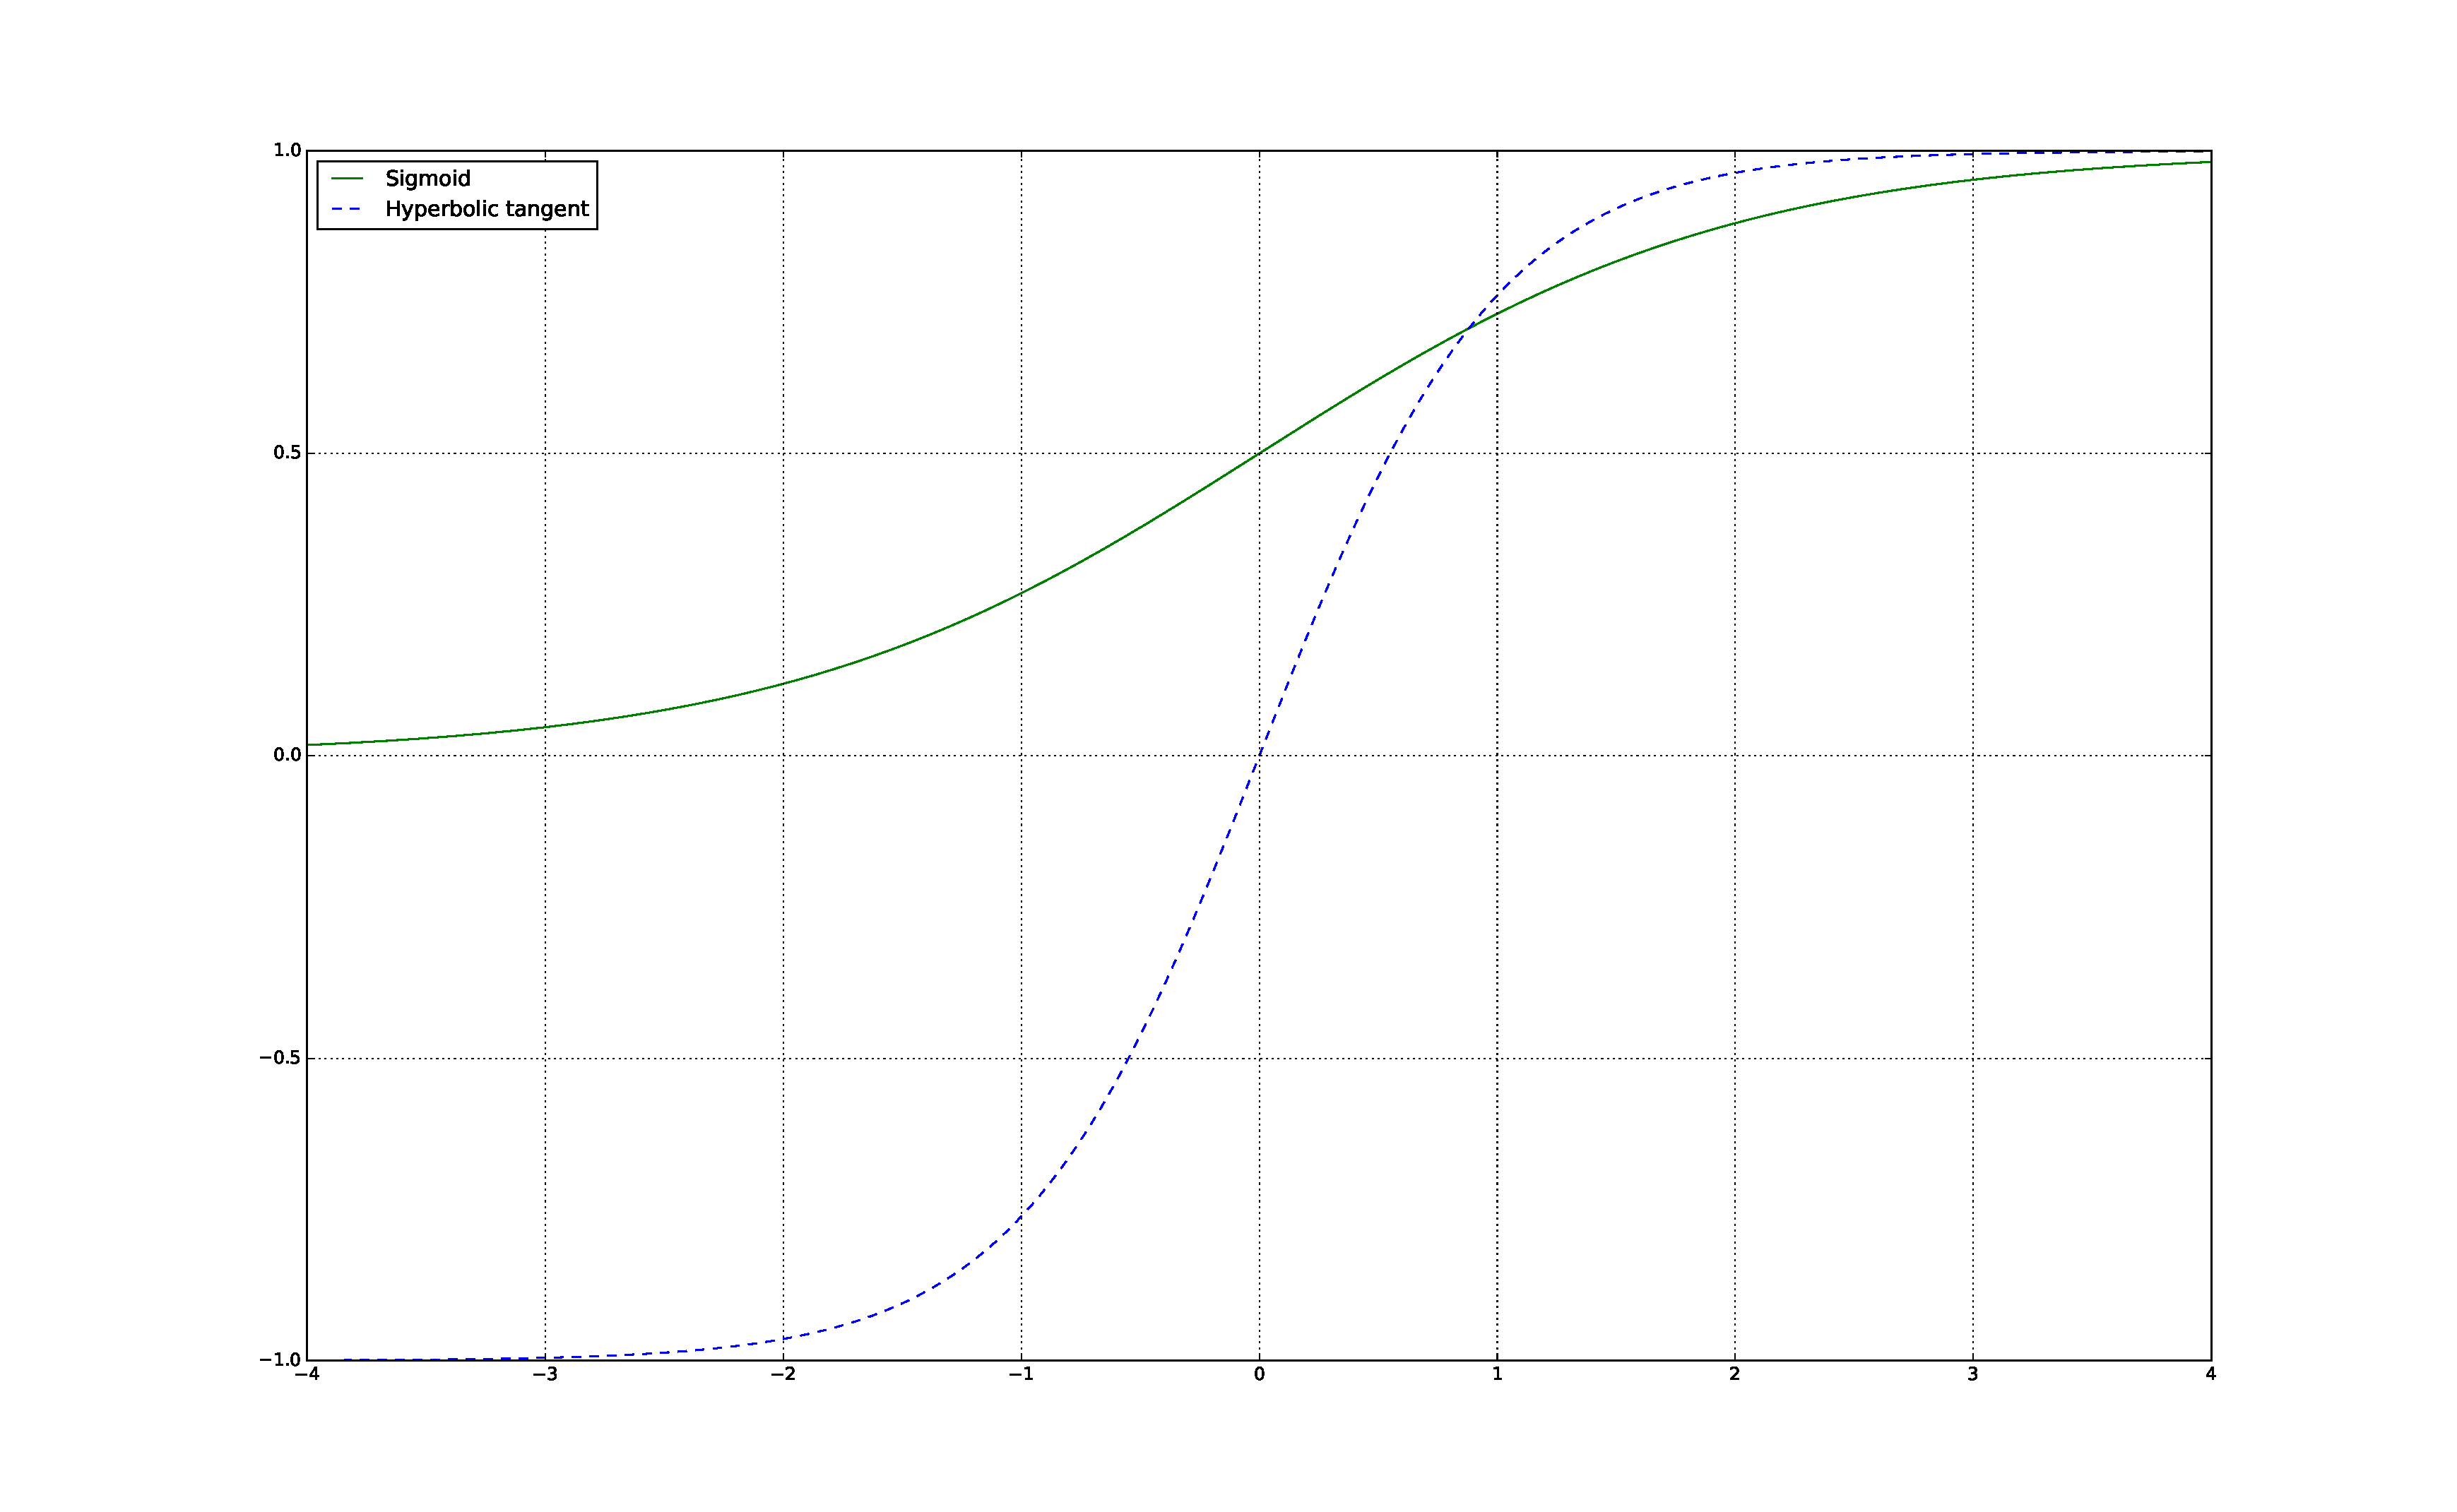
\includegraphics[width = 0.7\linewidth]{Figures/Theory/activationFunctions.pdf}
  \caption{Activation functions}
  \label{fig:activations}
  \end{center}
\end{figure}
Both these functions (Figure \ref{fig:activations}) have the desired properties mentioned above:
They are constant (1 or 0) for all values except a small interval around zero, where they have non-linear behaviour. 
This keeps the outputs of the neurons from blowing up. The sigmoid are more bilogically plausible because 
the output of inactive neurons are zero. Such activation function are called \textit{one-sided}. However,
it has been shown \cite{ref5} that the hyperbolic tangent 
performs better than the sigmoid for multi-layer networks. Nevertheless, one should assess the problem 
at hand when deciding what activation function to use; the performance can vary from problem to problem. 
(VENTE MED Å DISKUTERE DETTE TIL JEG HAR SNAKKET OM BACKPROPAGATION OSV.)
SNAKKE OM SATURATION OSV. 

In later years, the rectifier function (Figure \ref{fig:rectifier})
\begin{equation}
 f(x) = \max(0,x)
\end{equation}
has become the most popular for deep neural networks \cite{ref6}. PLOT DENNE FUNKSJONEN.
The two former functions are symmetrical around zero osv....
It have been argued to be even more biologically plausible than the sigmoid and also perform better
than the hyperbolic tangent for deep NNs. \cite{ref7}. 


A linear activation function $f(x) = x$ is often used in the output layer to avoid any constraint in the range 
of output values. For regression, the most widely used output activation is the unity function $f(x) = 1$, i.e.
no activation (HVORFOR?).

As shown in \eqref{completeNN}, the NN consists of several nested terms of the form
\begin{equation}
 h(x) = c_1 f(c_2 x + c_3) + c4
\end{equation}
where the parameters $c_i$ are weights and biases. By adjusting these parameters, the activation functions
can be shifted up and down or left and right, change slope or be rescaled, thus making the NN more flexible.

\subsection{Training}
The ability of the NN to represent a function accurately depends on the values of the weights. 
The weights are typically initialized as random numbers, and then optimized iteratively to minimize the error
to a set of expected output values. The expected output values are in our case known energies of a set of atomic
configurations, which have been obtained in quantum mechanical calculations of electronic structure. 
This optimization is called \textit{training} and an iteration is called an \textit{epoch}. 
The fitting process corresponds to the minimization of an error function, also known as the quadratic \textit{cost} function
\begin{equation}
 \Gamma = \frac{1}{2N}\sum_{i=1}^N (E_{i,ref} - E_{i,NN})^2
 \label{quadraticCostFunction}
\end{equation}
$E_{i,ref}$ are the known target energies, while $E_{i,NN}$ are the energies produced by the network. 
The constant $1/2$ are there to cancel out the exponent when we differentiate later. 
Other cost functions are used for other ML tasks (SKRIVE OM DISSE. KANSKJE HELE DENNE SEKSJONEN BØR 
SKRIVES MER GENERELL OG IKKE KUN FOR TILFELLET PES?)

\subsubsection{Backpropagation}
From: https://www.willamette.edu/~gorr/classes/cs449/backprop.html and \newline
http://neuralnetworksanddeeplearning.com/chap2.html. 
Mainly from the first one, but argument for error of neuron from second.

There are a large number of algorithms that can be used to determine the set of weights minimizing the 
cost function \eqref{quadraticCostFunction}. 
Different kinds of gradient descent methods are widely used, but to implement these we need the partial derivatives of
the cost function w.r.t. to all weights and biases to determine how we should adjust each weight. The idea behind gradient descent 
methods is to minimize a function by iteratively taking steps in the direction of the negative of its gradient w.r.t. 
all its parameters, i.e. the direction of steepest descent towards a minima:
\begin{equation}
 w_{ij}^{new} = w_{ij}^{old} - \gamma \frac{\partial \Gamma}{\partial w_{ij}^{old}}
 \label{gradientDescent}
\end{equation}
where we have skipped the layer indicies for clarity. Also, $w_{ij}$ now denotes the weight connecting node $j$ 
in layer $k$ with node $i$ in the following layer. This change of order is introduced to make it easier
to rewrite the below equations for backpropagation into matrix-vector equations. 
As seen from \eqref{gradientDescent}, we need to adjust each weight by an amount
\begin{equation}
\Delta w_{ij} = \frac{\partial \Gamma}{\partial w_{ij}}
\label{weightChange}
\end{equation}
The corresponding expression for the biases is
\begin{equation}
 \Delta b_i = \frac{\partial \Gamma}{\partial b_i}
\end{equation}
A common method to obtain these derivatives is backpropagation \cite{ref8}. 
In backpropagation, the output of the NN is compared to the desired output, the error is then propagated backwards
to adjust the weights. The method is essentially an implementation of the chain rule, and will allow us to calculate
the partial derivatives of the cost with respect to all the weights, thereby obtaining the gradient of the network. 

To change the value of the cost function \eqref{costFunction}, we need to change the outputs of the neurons in the network. 
Changing the input to neuron $j$ by a small amount $\Delta x_j$ results in the output
\begin{equation}
 y_j = f_j(x_j + \Delta x_j)
 \label{neuronError}
\end{equation}
This change will propagate through later layers in the network, finally causing the overall cost to change
by an amount $\frac{\partial \Gamma}{\partial x_j}\Delta x_j$. If $\partial \Gamma / \partial x_j$ is close to zero,
then we can't improve the cost much by perturbing the weighted input $x_j$; the neuron is already quite near the optimal value.
This is a heuristic argument for $\partial \Gamma / \partial x_j$ to be a measure of the error of the neuron:
\begin{equation}
 \delta_j \equiv \frac{\partial \Gamma}{\partial x_j}
\end{equation}
We also define
\begin{equation}
 A_i = \{j:w_{ij}\}
\end{equation}
as the set $\{j\}$ of nodes anterior to node $i$ and connected to node $i$ with weights $w_{ij}$, in addition to
\begin{equation}
 P_j = \{i:w_{ij}\}
\end{equation}
as the set $\{i\}$ of nodes posterior to node $j$ and connected to node $j$ with weights $w_{ij}$. 

The weight change \eqref{weightChange} can be expanded into two factors by use of the chain rule:
\begin{equation}
 \Delta w_{ij} = \frac{\partial \Gamma}{\partial x_i}\frac{\partial x_i}{\partial w_{ij}}
\end{equation}
Now we move in the opposite direction compared to the feed-forward function composition stage: First we differentiate the cost w.r.t 
neuron $i$'s input, then we differentiate the input w.r.t. weight $w_{ij}$ connecting neurons $j$ and $i$. The first term on the right
is the error $\delta_i$ of node $i$. The second is
\begin{equation}
 \frac{\partial x_i}{\partial w_{ij}} = \frac{\partial}{\partial w_{ij}} \sum_{m\in A_i} w_{im}y_m = y_j
\end{equation}
Putting the two together, we get
\begin{equation}
 \Delta w_{ij} = \delta_i y_j
\end{equation}
To compute this quantity, we thus need to know the output and the error for all nodes in the network. 
The outputs are as we have seen
\begin{equation}
 y_i = f_i(x_i) = f_i\left(\sum_{j\in A_i} w_{ij}y_j + b_i\right)
 \label{forwardProp}
\end{equation}
The error for output neuron $o$ is
\begin{equation}
 \delta_o = \frac{\partial \Gamma}{\partial x_o} = \frac{\partial \Gamma}{\partial y_o}\frac{\partial y_o}{\partial x_o}
          = (d_o - f_o(x_o)) \frac{\partial f_o(x_o)}{\partial x_o}
\end{equation}
When doing regression our output neurons will have the unity activation function, which means that the error is reduced to
\begin{equation}
 \delta_o = d_o  - y_o
\end{equation}
This error is then propagated backwards through the network. Each hidden neuron will have an error
\begin{equation}
 \delta_j = \frac{\partial \Gamma}{\partial x_j} = 
 \sum_{i\in P_j} \frac{\partial \Gamma}{\partial x_i}\frac{\partial x_i}{\partial y_j}\frac{\partial y_j}{\partial x_j}
 \label{errorTerms}
\end{equation}
The first term on the right is the error of node $i$. The second is the derivative of the net input of all posterior
nodes $\{i\}$ w.r.t. the output of node $j$:
\begin{equation}
 \frac{\partial x_i}{\partial y_j} = \frac{\partial}{y_j}\left(\sum_{m\in A_i} w_{im}y_m + b_i\right) = w_{ij}
\end{equation}
while the third is the derivative of node $j$'s activation function w.r.t. its net input:
\begin{equation}
 \frac{\partial y_j}{\partial x_j} = \frac{\partial f_j(x_j)}{\partial x_j} \equiv f_j^\prime (x_j)
\end{equation}
Putting all the pieces together we obtain
\begin{equation}
 \delta_j = f_j^\prime(x_j)\sum_{i\in P_j} \delta_i w_{ij}
 \label{backProp}
\end{equation}
The above expression requires that we know the errors of all the posterior nodes
of node $j$. As long as there are no cycles in the network, there is an ordering of nodes from the output back to the 
input that respects this condition. It is therefore valid only for feed-forward NNs.
The errors are propagated backwards through the whole NN until we reach the input nodes. By propagating the error
of only one ouput neuron, we thus obtain the errors of all the neurons at once. This is the strength of the backpropagation
algorithm. 
For the biases, we have
\begin{equation}
 \Delta b_j = \frac{\partial \Gamma}{\partial b_j} = \sum_{i\in P_j} \frac{\partial \Gamma}{\partial x_i}
	      \frac{\partial x_i}{\partial y_j} \frac{\partial y_j}{\partial x_j} \frac{\partial x_j}{\partial b_j}
\end{equation}
The only new term her is the last one:
\begin{equation}
 \frac{\partial x_j}{\partial b_j} = \frac{\partial}{\partial b_j}\left(\sum_{m\in A_j} w_{jm}y_m + b_j\right) = 1
\end{equation}
Consequentially, the update rule for the biases is simply the error of each neuron:
\begin{equation}
 \Delta b_j = \delta_j
\end{equation}
For fully-connected FFNNs we can easily rewrite these equations in matrix notation. In this notation, 
the biases, inputs, outputs and errors for all nodes in a layer are combined into vectors, while all weights from 
one layer to the next form a matrix $W_l$, where $l$ denotes the layer number. The inputs to all the nodes in 
layer $l$ can be written
\begin{equation*}
    \left(\begin{array}{c}
            x_1^l \\
            x_2^l \\
            x_3^l \\
          \end{array} \right)
 = \left(\begin{array}{c c c}
            w_{11} & w_{12} & w_{13} \\
            w_{21} & w_{22} & w_{23} \\
	    w_{31} & w_{32} & w_{33} \\
   \end{array} \right)
   \left(\begin{array}{c}
            y_1^k \\
            y_2^k \\
            y_3^k \\
         \end{array}\right)
 + \left(\begin{array}{c}
          b_1^l \\
          b_2^l \\
          b_3^l \\
         \end{array}\right)
\end{equation*}
so that equation \eqref{forwardProp} takes the form
\begin{equation}
\vec{y}_l = f_l(W_l\vec{y}_{l-1} + \vec{b}_l)
\end{equation}
Comparing equations \eqref{forwardProp} and \eqref{backProp}, we observe that 
\begin{equation}
 \sum_{j\in A_i}w_{ij} = \left(\sum_{i\in A_j}w_{ij}\right)^T
\end{equation}
i.e. the weight matrices used in backpropagation are the transpose of the matrices used in forward activation.
The complete backpropagation algorithm including forward activation then looks as follows:
\begin{enumerate}
 \item Initialize the input layer:
 \begin{equation}
  \vec{y}_0 = \vec{x}_0
 \end{equation}
 \item Propagate the activity forward: for $l = 1,2,\dots ,L$:
 \begin{equation}
  \vec{y}_l = f_l(W_l\vec{y}_{l-1} + \vec{b}_l)
 \end{equation}
 \item Calculate the error in the output layer:
 \begin{equation}
  \vec{\delta}_L = \vec{t} - \vec{y}_L
 \end{equation}
 \item Calculate the error: for $l = L-1, L-2, \dots ,1$:
 \begin{equation}
 \vec{\delta}_l = (W^T_{l+1}\vec{\delta}_{l+1}) \cdot f_l^\prime (\vec{x}_l)
 \end{equation}
 \item Update the weights and biases: 
 \begin{equation}
  \Delta W_l = \vec{\delta}_l \vec{y}_{l-1}^T, \quad \Delta \vec{b}_l = \vec{\delta}_l
 \end{equation}
\end{enumerate}


\section{Neural networks in molecular dynamics}
Following \cite{ref9} and \cite{ref10}.
All the dynamics of a molecular system is determined by the multidimensional potential-energy surface (PES), which
in general is a real-valued function depending on all atomic coordinates in the system. Using the Born-Oppenheimer approximation
(FORKLARE ELLER REFERERE), 
various quantum mechanical methods like Hartree-Fock and density functional theory (DFT) are available to directly calculate
the PES and forces for a given configuration. Calculating the energies for all relevant configurations of a system is
demanding and time-consuming, and only a limited number of energies can be computed and stored. 
Consequentially, during a \textit{ab inito} molecular dynamics (MD) simulations, the energies and forces for all configurations visited
are not available beforehand. In \textit{ab inito} MD, energies and forces are therefore calculated on-the-fly, typically using DFT.
This is however a very inefficient approach. A more efficient method is to construct an analytical PES to use in simulations, 
but this can only be done for very simple systems.

A solution to this problem is the introduction of approximate PESs, and there are two fundamental approaches. 
The most widely used and convential method is to replace the solution of the Schrödinger equation by a simplified
energy expression based on physical considerations and reasonable approximations. These functions are not obtained
by ab inito methods, but can in many cases be sufficiently accurate to be used in simulations (BØR HA EN EGEN SEKSJON
OM DE VANLIGSTE POTENSIALENE).

An alternative approach is to employ machine learning (ML) potentials that have no direct physical meaning. 
The aim of these purely mathematical functions is to fit an analytic expression to a set of reference data
obtained by quantum mechanical calulations. There are various methods (REFERENCES). 
ML potentials are particularly useful
\begin{itemize}
 \item if long MD simulations are required
 \item if many MD trajectories are needed
 \item if the systems are too large for the application of QM methods
\end{itemize}
Physical and ML potentials thus enables us to extend the time and length scales of MD simulations
beyond the realm of ab inito methods. 

Feed-forward neural networks (FFNN) have been demonstrated to be useful for the construction of PESs because
they are universal function approximators. There is no restriction in the accuracy that can be achieved when 
constructing neural network potentials (NNP). Unlike physical potentials, they are not restricted by any \textit{ad hoc}
functional form. NNPs offer a number of advantages for the construction of PESs:
\begin{itemize}
 \item Energies can be fitted to very high accuracy, leaving only
 the underlying error of the reference data
 \item Evaluation of NNPs require much less CPU time than QM methods
 \item The NNP expression is unbiased and generally applicable to all types of bonding
\end{itemize}
Still, there are disadvantages one should be aware of:
\begin{itemize}
 \item The evaluation of NNPs are notably slower compared to the use of classical force fields
 \item NNP expressions have no physical interpretation, and have very limited extrapolation capabilities
 \item NNPs are, for the time being, only applicable to systems containing only a few
 different chemical elements (but many atoms)
\end{itemize}

\subsection{High-dimensional NNPs}
The use of a single FFNN to represent complicated systems containing many atoms of different types is not possible for several reasons.
First of all, the deegrees of freedom (the number of weight parameters) will be very many, making the training and evaluation
of the network slow. Secondly, the NN has a symmetry problem. It does not take into account that exchanging two or more atoms
can lead to an energetically equivalent configuration. For example, exchanging the positions of both hydrogen atoms
in a water molecule will not alter the configuration energy. However, noting that all weights have numerically different values,
changing the order of the input coordinates to the NN will result in a different energy value. This problem can be solved
by a different choice of input coordinates, discussed below. The third problem in using a single FFNN is that it is 
only applicable to the system size that has been used during the training. If the NN has been trained with 5 inputs, 
it can not be used for a system containing any other number of atoms. 
\begin{figure}[H]
\begin{center}
  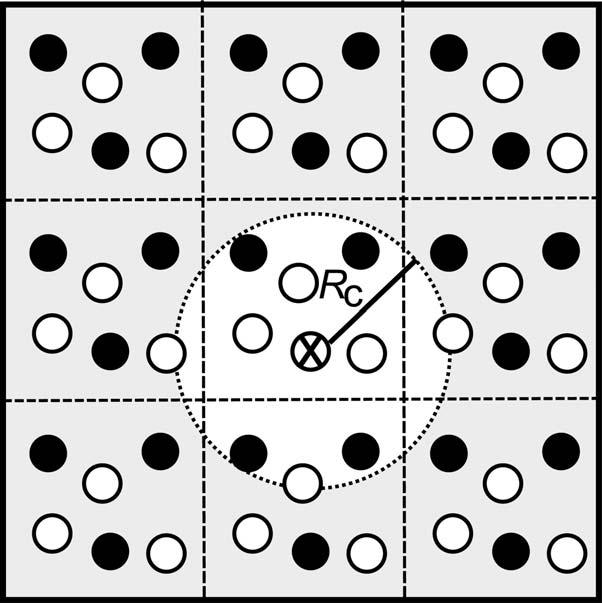
\includegraphics[width = 100mm]{Figures/Theory/cutOffHighDimNN.jpeg}
  \caption{}
  \label{fig:cutOffNeighbours}
  \end{center}
\end{figure}
A solution to all these problems is to construct the system energy $E_s$ as a sum of $N$ atomic energy contributions
$E_i$, which are provided by a set of individual atomic NNs,
\begin{equation}
 E_s = \sum_{i=1}^N E_i
\end{equation}
The atomic energies $E_i$ depend on the local chemical environment up to a cutoff radius $R_c$ as shown in figure
\ref{fig:cutOffNeighbours} (STJÅLET FRA PAPER, MÅ LAGE EGEN?). 
This is analogous to MD simulations with neighbour lists, thus making it possible to 
obtain the energies and forces of an atom and all its neighbours simultaneously. The positions of the neighbouring atoms within 
the cutoff sphere are described by a set of many-body symmetry functions discussed below. As the order of the summation does not 
change the total energy $E_s$, the symmetry problem above is solved. Each chemical element have seperate types of
NNs with their own architecture and weights, but for a given element all atomic NNs are equal. Such a system of NNs are also 
applicable to different system sizes: To add an atom of a given type, we simply extend the set of NNs by another network
identical to the other NNs of the same type, and if an atom is removed, we delete the respective NN. 
\begin{itemize}
 \item The introduction of the cutoff $R_c$ reduces the effective dimensionality
 of the problem, which allows to use NNs of tractable size
 \item The total energy is invariant with respect to the order of the atoms
 \item The NNP can be used for systems of different sizes
 \item We 
\end{itemize}
We know that the energy of a molcule does not change under a translation or a rotation. Thus our symmetry functions
should be invariant with respect to these operations. 

\subsection{Symmetry functions}
To construct adequate symmetry functions, we need to have a cutoff function that defines the atomic environments. 
One such function is \cite{ref9},
\begin{equation}
 f_c(R_{ij}) = 
\begin{cases}
0.5 \cdot \left[\cos\left(\frac{\pi R_{ij}}{R_c}\right) + 1 \right], & R_{ij} \leq R_c \\
0, & R_{ij} > R_c
\end{cases}
\label{cutoffFunction}
\end{equation}
which is the monotonically decreasing part of a cosine function on $R_{ij} \in [0,R_c]$, seen in \autoref{fig:cutoffFunction}. 
\begin{figure}[H]
\begin{center}
  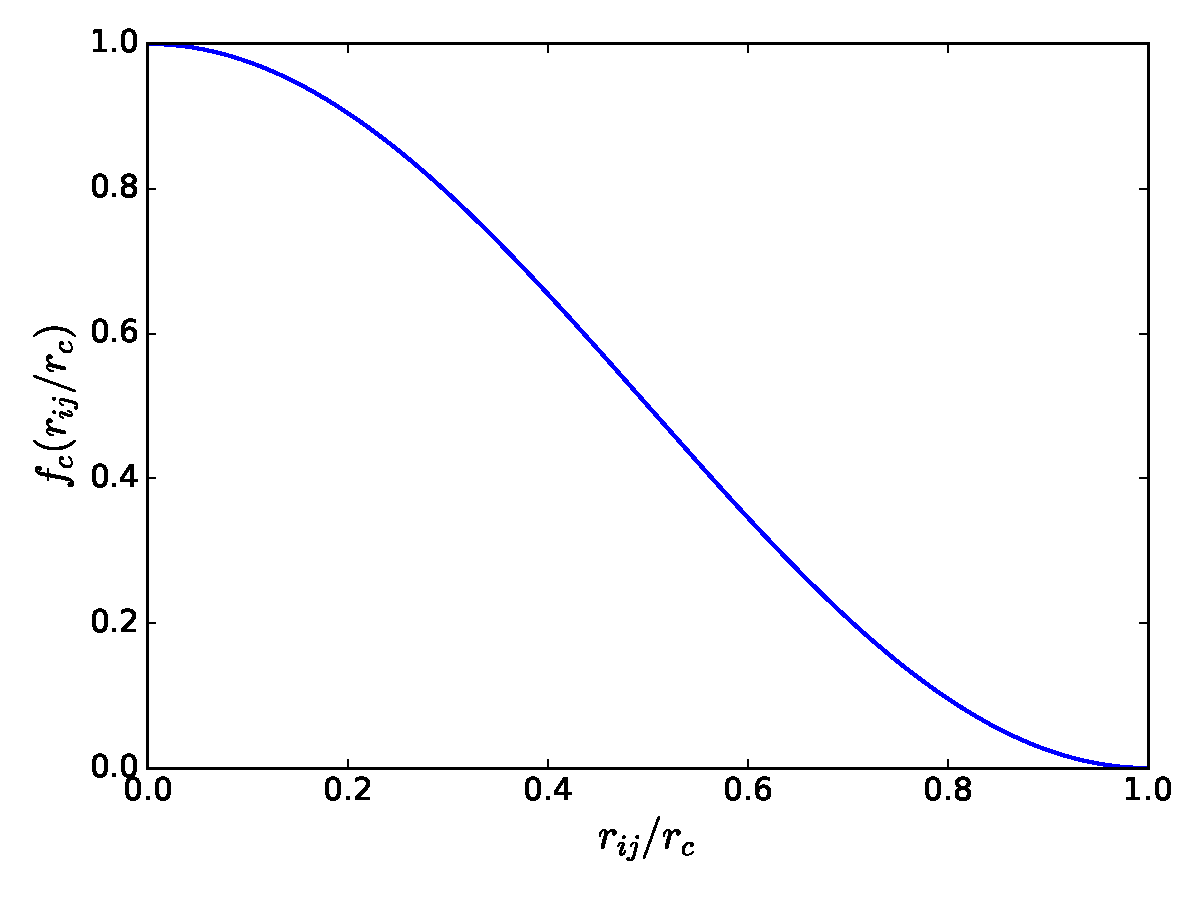
\includegraphics[width = 0.9\linewidth]{Figures/Theory/cutoffFunction.pdf}
  \caption{Plot of the cutoff function \eqref{cutoffFunction} applied in this thesis. 
	   This function is used to define a chemical environment around a central atom:
           only the atoms within the cutoff radius $R_c$ contribute to its energy. 
           These are called neighbouring atoms. The closer a neighbouring atom is, the larger
           the energy contribution, as is the case for most physical systems.}
  \label{fig:cutoffFunction}
  \end{center}
\end{figure}
This function have the desirable property that it decreases with increasing distance $R_{ij}$ between the central
atom $i$ and its neighbour $j$. At the cutoff radius $R_c$, is has zero value and slope, which is important
to avoid discontinuities when computing energies and forces. Atoms beyond the cutoff radius are not a part of the central
atom's chemical environment and therfore do not contribute to its energy. 

Several types of many-body symmetry functions can be
constructed based on these cutoff functions. They can be divided into two classes: \textit{radial} symmetry functions, describing 
the radial distribution of neighbours up to the cutoff radius, and \textit{angular} symmetry functions, specifying their
angular arrangement. All symmetry functions depend on the positions of all the atoms inside the cutoff spheres. They make
it possible to obtain a constant number of function values independent of the number of neighbours, which can change
during MD simulations. 

The most basic radial symmetry function is simply the sum of the cutoff functions for all the neighbours $j$ to 
atom $i$,
\begin{equation}
 G_i^1 = \sum_{j=1}^N f_c(R_{ij})
 \label{G1}
\end{equation}
We need a set of such functions with different cutoff radii to describe the radial arrangement of the neighbouring atoms. 
A better alternative is to use a sum of products of Gaussians and the cutoff function,
\begin{equation}
 G_i^2 = \sum_{j=1}^N \exp[-\eta(R_{ij}-R_s)^2] \cdot f_c(R_{ij})
 \label{G2}
\end{equation}
We now have two parameters that can be adjusted to probe different radii. The width parameter $\eta$ determines the 
radial extension of the symmetry functions, while the shifting parameter $R_s$ displaces the Gaussians to improve
the sensitivity of the symmetry functions at specific radii. A third option is 
\begin{equation}
 G_i^3 = \sum_{j=1}^N \cos(\kappa R_{ij}) \cdot f_c(R_{ij})
 \label{G3}
\end{equation}
which are damped cosine functions with a period length adjusted by parameter $\kappa$. We will however not use 
this function because of the existence of negative function values which can lead to atoms canceling each other's
contribution to the sum. In \autoref{fig:radialSymmetriFunctions} we see the radial symmetry functions for several
different parameters. It is clear that a set of such functions have a large flexibility when we tune the parameters
in different ways. This is what makes them able to represent the radial distribution of neighbours around a central atom. 
\begin{figure}[H] 
  \begin{subfigure}[b]{0.5\linewidth}
    \centering
    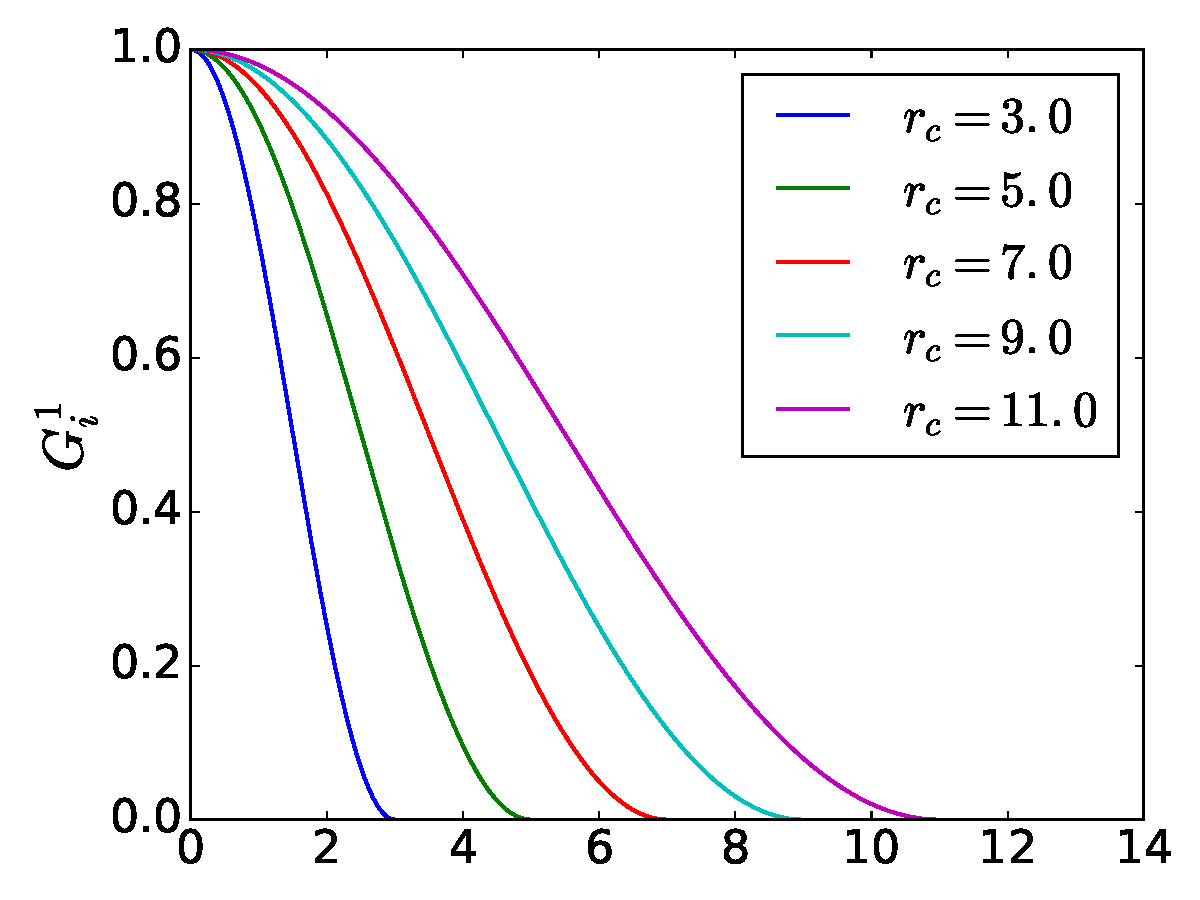
\includegraphics[width=\linewidth]{Figures/Theory/G1.pdf} 
    \label{fig:radialSymmetriFunctions:a} 
    \vspace{1ex}
  \end{subfigure}%% 
  \begin{subfigure}[b]{0.5\linewidth}
    \centering
    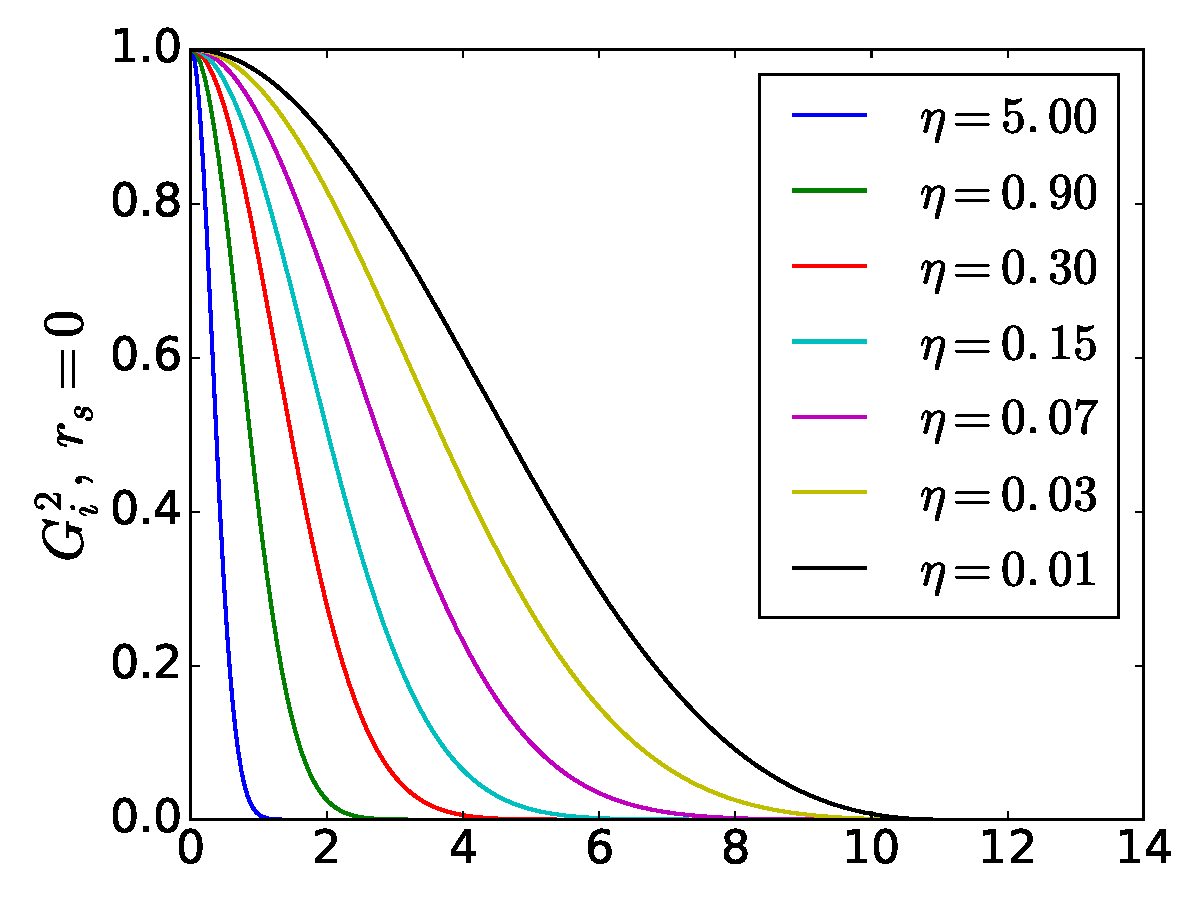
\includegraphics[width=\linewidth]{Figures/Theory/G2_1.pdf} 
    \label{fig:radialSymmetriFunctions:b} 
    \vspace{1ex}
  \end{subfigure} 
  \begin{subfigure}[b]{0.5\linewidth}
    \centering
    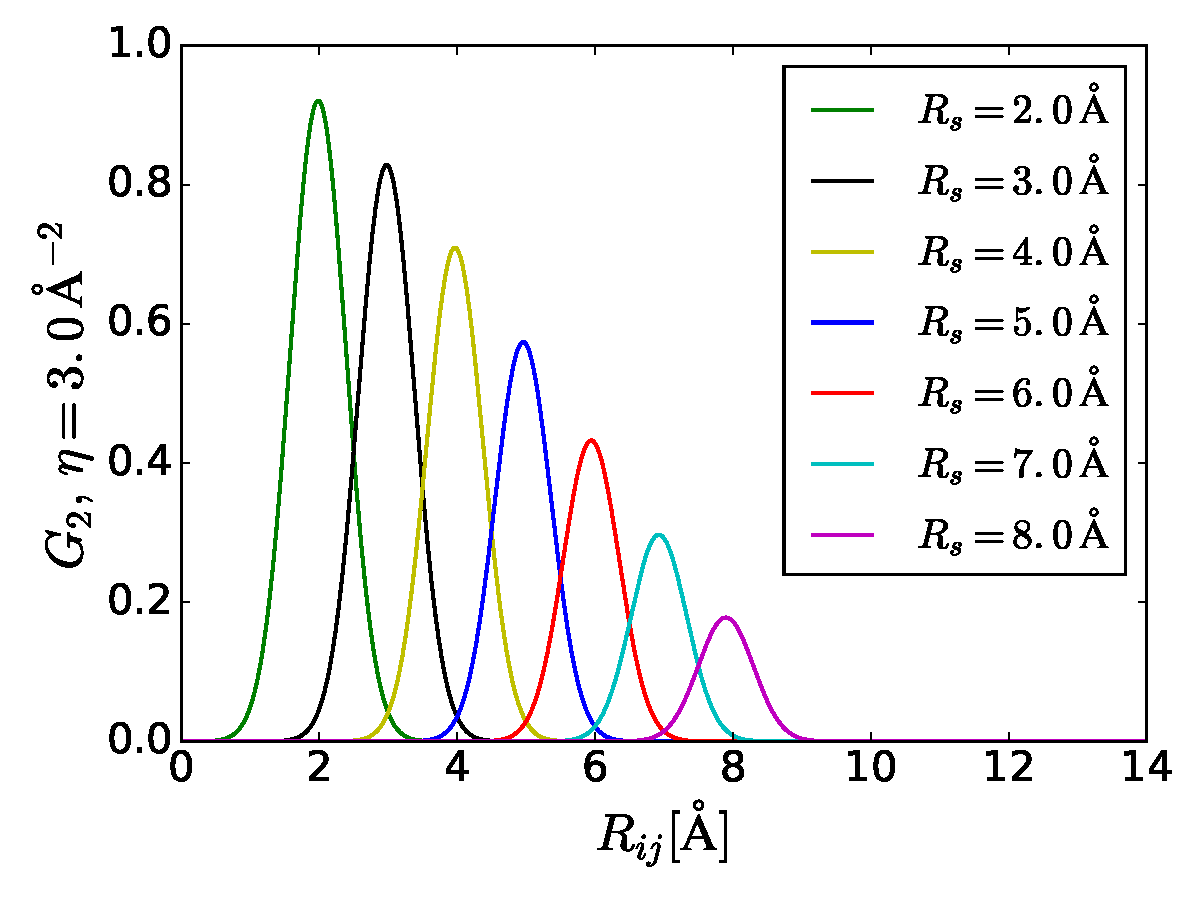
\includegraphics[width=\linewidth]{Figures/Theory/G2_2.pdf} 
    \label{fig:radialSymmetriFunctions:c} 
  \end{subfigure}%%
  \begin{subfigure}[b]{0.5\linewidth}
    \centering
    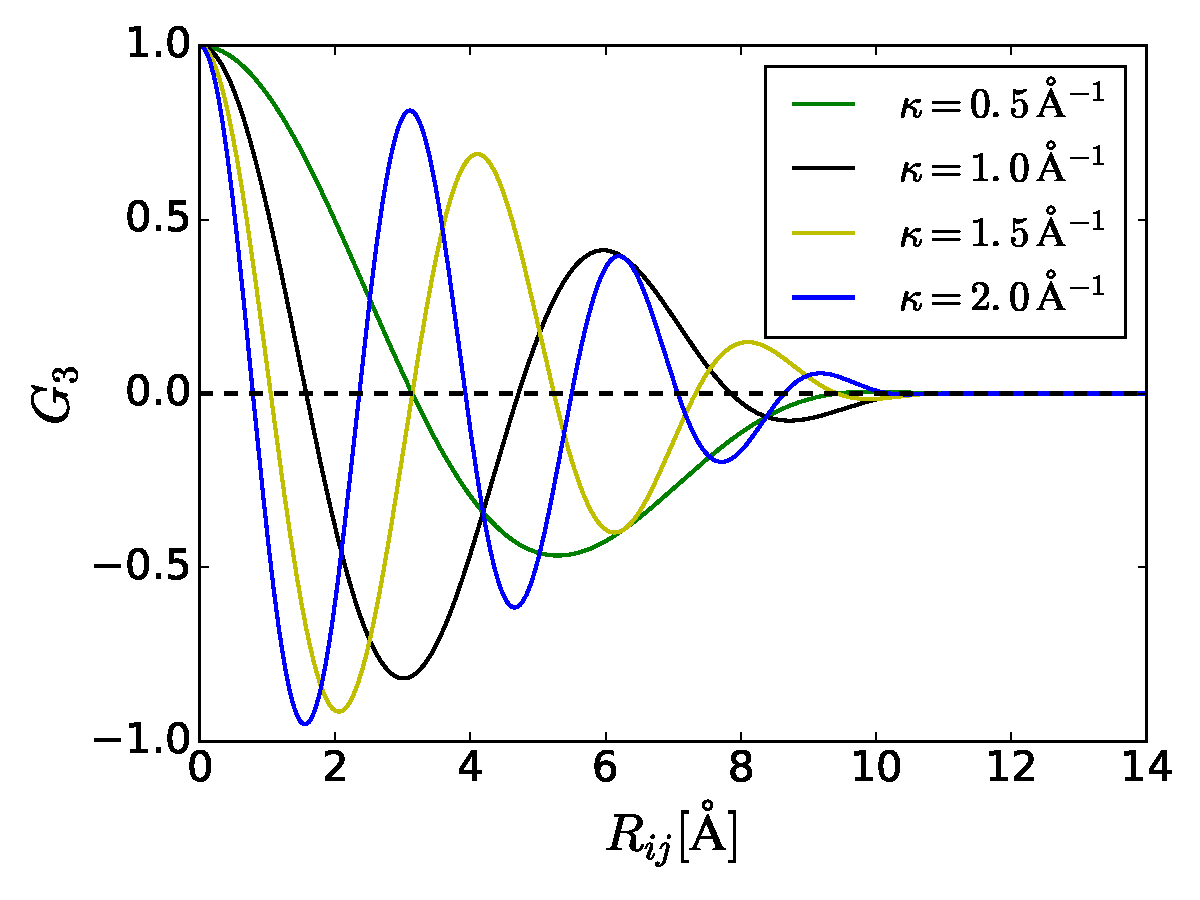
\includegraphics[width=\linewidth]{Figures/Theory/G3.pdf} 
    \label{fig:radialSymmetriFunctions:d} 
  \end{subfigure} 
  \caption{Radial symmetry functions $G^1$, $G^2$ and $G^3$ for an atom with one neighbour only. A set of such 
	   functions represents the radial distrubution of neighbours around a central atom placed at the origin.
	   For $G^2$ and $G^3$ a cutoff $R_c = \SI{11.0}{\angstrom}$ has been used.}
  \label{fig:radialSymmetriFunctions} 
\end{figure}
To obtain a suitable structural fingerprint of the atomic environments, we also need the angular distribution
of neighbouring atoms. This can be achieved by using functions depending on $\theta_{ijk}$, which
is the angle formed by the central atom $i$ and the two interatomic distances $R_{ij}$ and $R_{ik}$. 
The potential is periodic with respect to this angle, so we can use the cosine of $\theta_{ijk}$ instead. 
We thus define an angular symmetry function as a sum over all cosines with respect to any possible pair of 
neighbours $j$ and $k$, multiplied by Gaussians of the three interatomic distances and the respective cutoff functions,
\begin{align}
 G_i^4 = 2^{1-\zeta}\sum_{j\neq i}\sum_{k>j} &[(1 + \lambda \cos\theta_{ijk})^\zeta \cdot
 \exp(-\eta (R_{ij}^2 + R_{ik}^2 + R_{jk}^2)) \cdot \\
 &f_c(R_{ij}) f_c(R_{ik}) f_c (R_{jk})]
 \label{G4}
\end{align}
This function becomes zero if any of the interatomic distances is larger than $R_c$. The parameter $\eta$ takes here
into account that the angular contribution depends on the atomic seperations. The angular arrangement can be 
investigated by using different values for $\zeta$ while the normalization factor $2^{1-\zeta}$ ensures that the range of 
values is independent of the choice of $\zeta$. The parameter $\lambda \in {-1,1}$ can be used to invert the shape of the 
cosine function: for $\lambda = +1$ the maxima of the cosine terms are at $\theta_{ijk} = 0^\circ$, 
while for $\lambda=-1$ they are located at $\theta_{ijk} = 180^\circ$. The cutoff function $R_{jk}$
is included to ensure that only triplets where all three inter-atomic distances are within the cutoff radius. 
Another function can be defined that has no constraint on $R_{jk}$,
\begin{align}
  G_i^5 = 2^{1-\zeta}\sum_{j\neq i}\sum_{k>j} &[(1 + \lambda \cos\theta_{ijk})^\zeta \cdot
 \exp(-\eta (R_{ij}^2 + R_{ik}^2)) \cdot \\
 &f_c(R_{ij}) f_c(R_{ik})]
 \label{G5}
\end{align}
\eqref{G5} will generally have larger function values than \eqref{G4} because the lack of constraint on $R_{jk}$ results in 
a larger number of non-zero terms in the summation. The angular part of $G^4$ and $G^5$ is identical, shown in 
\autoref{fig:angularSymmetryFunctions} for different values of $\zeta$. 
\begin{figure}[H]
  \begin{subfigure}[b]{0.5\linewidth}
    \centering
    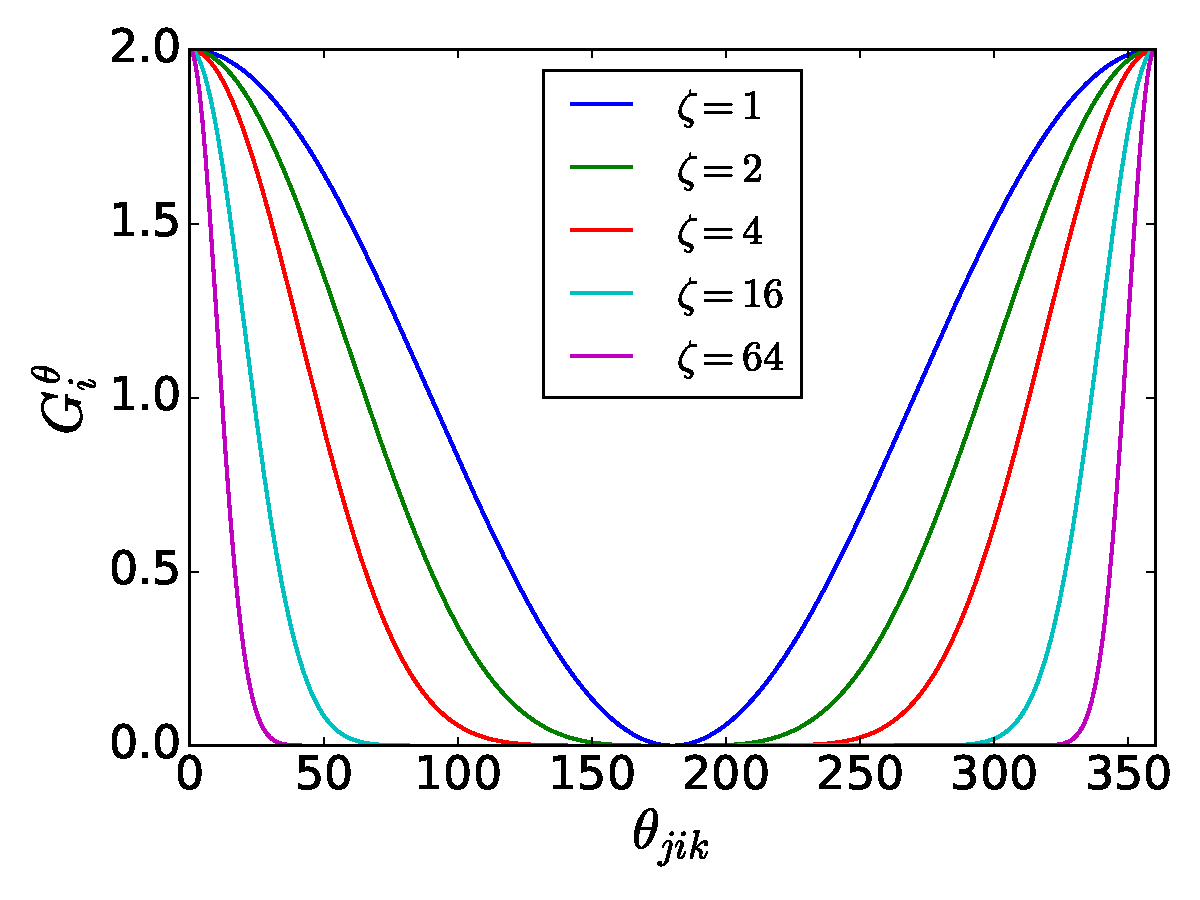
\includegraphics[width=\linewidth]{Figures/Theory/G4G5angular1.pdf}
    \subcaption{}
    \label{fig:angularSymmetryFunctions:a} 
  \end{subfigure}%% 
  \begin{subfigure}[b]{0.5\linewidth}
    \centering
    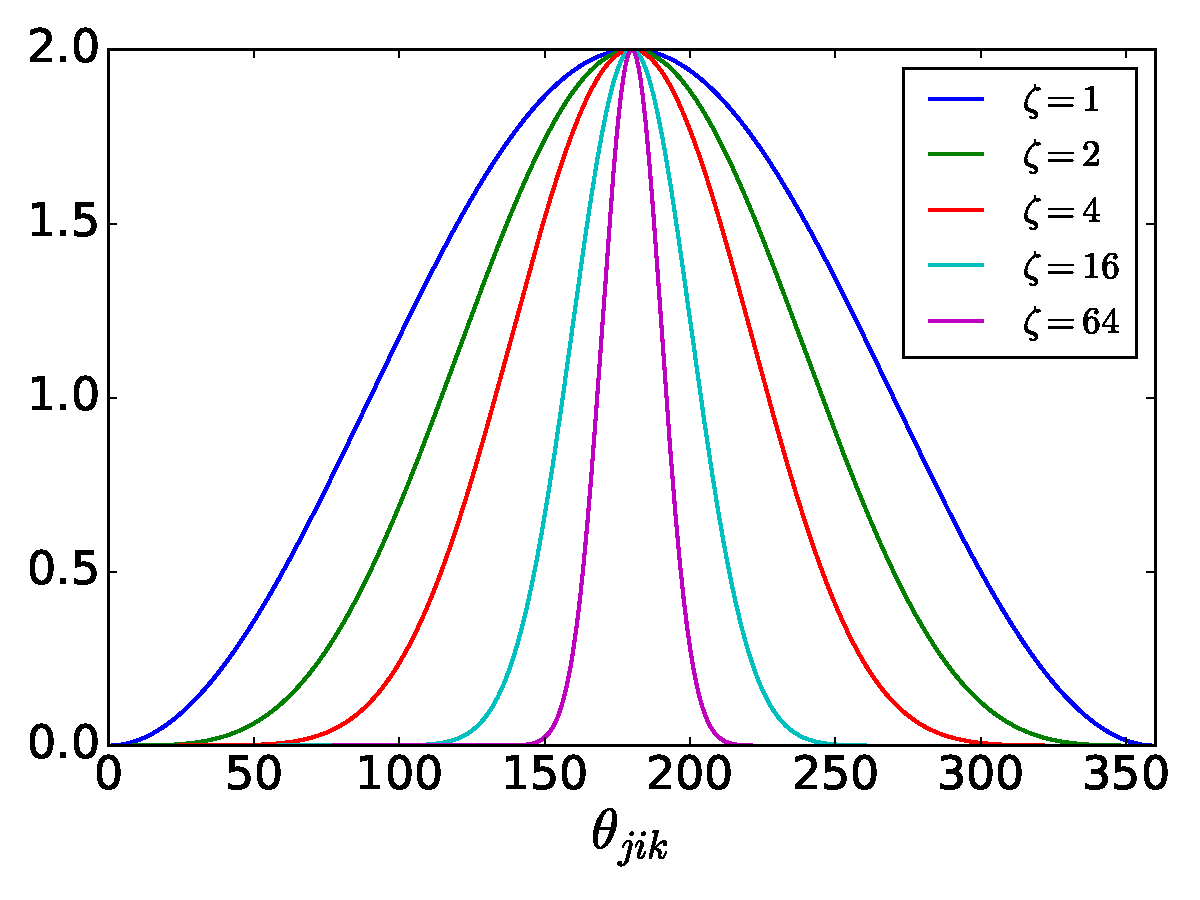
\includegraphics[width=\linewidth]{Figures/Theory/G4G5angular2.pdf} 
    \subcaption{}
    \label{fig:angularSymmetryFunctions:b} 
  \end{subfigure} 
  \caption{Angular part of symmetry functions $G^4$ and $G^5$ for an atom with one neighbour only. A set of such 
	   functions represents the angular distrubution of neighbours around a central atom placed at the origin.
	   $\lambda = +1$ for \autoref{fig:angularSymmetryFunctions:a}, $\lambda=-1$ for \autoref{fig:angularSymmetryFunctions:b}.}
 \label{fig:angularSymmetryFunctions} 
\end{figure}
The parameter values $R_c, \eta, R_s, \zeta$ and $\lambda$ are not automatically optimized, like the weights. 
Once a set of symmetry functions has been determined, they remain fixed during the training of the NN. They are therefore
an integral part of the NN, and need to be evaluated together with the NN itself when applied in simulations. 
The symmetry function set have to be customized for different systems, but in our experience the quality of the fit 
is not very sensitive to the choice of parameters. An adequate set will shorten the convergence time, but it will not 
necesseraly result in a lower RMSE. 
However, it is important to use at least as many symmetry functions as there are degrees of freedom in the system.
If this is not the case, the NN will recieve insufficient information and will not be able to fit the data properly. 

\subsection{Symmetry functions and forces}
To do MD simulations we need need the forces \eqref{forcePES}, i.e. the gradient of the PES. 
NNs have as we have seen well-defined functional forms, and analytical derivatives are therefore readily available.
The pair-force on the central atom $i$ from neighbour $j$ w.r.t som atomic coordinate $\alpha$ is
\begin{equation}
 F_{ij,\alpha} = -\frac{\partial E}{\partial \alpha_{ij}} = \sum_{\mu=1}^{M}\frac{\partial E}{\partial G_\mu}
 \frac{\partial G_\mu}{\partial \alpha_{ij}}
 \label{pairForce}
\end{equation}
where $\alpha_{ij} = \alpha_i - \alpha_j = \alpha_j$ and $M$ is the number of symmetry functions, i.e. the number
of inputs to the NN. As seen by the r.h.s of this equation, we need to apply the chain rule: The first term
$\partial E/\partial G_\mu$ is the derivative of the output ($E$) w.r.t. symmetry function number $\mu$, the second
term is the derivative of $G_\mu$ w.r.t. the atomic coordinate $\alpha$. The former is obtained with a slightly modified
form of backpropagation.
\begin{enumerate}
 \item Instead of backpropagating the error, we backpropagate the derivative of the output neuron's activation function
 \item The derivative is propagated all the way back to the input nodes. When training, the propagation
 stops at the weights of the first hidden layer. 
\end{enumerate}
This clarifies how a fully-connected feed-forward NN is built: To get the derivative of the output neuron
w.r.t. the input neurons, we have to also compute the derivative of all the neurons and weights in-between because
all nodes in each layer are connected to all nodes in the following layer. The term $\partial G_\mu/\partial \alpha_{ij}$
depends only on the form of the symmetry functions. See appendix for derivatives of these. Since all symmetry functions
$G_\mu$ depend on the atomic coordinates of all the neighbours, we have to sum over all the input nodes to get
the total force from neighbour $j$ on central atom $i$. 

The total force on atom $i$ is obtained by calculating \eqref{pairForce} for all neighbours and adding them,
\begin{equation}
 F_{i,\alpha}^{TOT} = -\sum_{j=1}^N
 \sum_{\mu=1}^{M}\frac{\partial E}{\partial G_\mu}
 \frac{\partial G_\mu}{\partial \alpha_{ij}}
\end{equation}
where $N$ is the number of neighbours. TODO: THIS EXPRESSION HAS TO BE MODIFIED A BIT IF I INCLUDE MORE THAN ONE ATOM TYPE.
THEN THE TOTAL ENERGY E WILL BE DIFFERENT DEPENDING ON WHICH ATOM TYPE EACH NEIGHBOUR IS AND SO ON...


\section{TensorFlow}
TensorFlow is an open source software library for numerical computation using data flow graphs (DFG). 
A DFG describe mathematical computations with a directed graph of nodes and egdes. Nodes typically represent mathematical
operations, while the graph edges describe the input/output relationship between nodes. In TensorFlow, these edges
carry dynamically-sized tensors, i.e. there is a flow of tensors between nodes in the graph. 

We train a neural network by introducing different variables at the nodes. We want to minimize the cross-entropy (error)
with respect to these variables. The derivatives of the output w.r.t. these are calculated using bacpropagation. These derivatives
are then used to minimize the cross-entropy using the gradient descent method or other optimization algorithms. 

TensorFlow uses ReLU neurons, i.e. the activation function is
\begin{equation}
 f(x) = \max(0,x)
\end{equation}
where $x$ is the input to the neuron. This is also known as a ramp function, or a rectifier (in analogy to half-wave
rectification in electrical engineering). 
The above function has lately been argued to be more biologically plausible (REFERENCE)
than the widely used sigmoid function and hyperbolic tangent. A smooth approximation to the rectifier is the analytic function
\begin{equation}
 f(x) = \ln(1 + e^x)
\end{equation}
which is called the softplus function. Using this kind of activation function prevents «dead neurons».
In practice we give initialize the neurons with a sligthly positive initial bias. 

\subsection{Convolution}
ANNs are supposed to mimic biological systems. We know that neurons in the visual cortex of animals have
localized receptive fields, i.e. they respond only to stimuli in a certain location of the visual field. 
These regions are overlapping and covers the entire visual field. This can be exploited in ANNs by making the hidden layers
only connect to a small contigous region of the input layer. This also speeds up computations. These are called
locally connected networks, unlike fully connected networks, where all the hidden layers are connected to the complete
input layer. 

Using this approach, we can aggregate statistics of these features at various locations. This is called pooling. 

\chapter{Verifications and tests}

\section{Time usage}
The workflow when training a NN and using it in MD is as follows: 
\begin{enumerate}
 \item Generate training data
 \item Train a NN to fit the data
 \item Use the analytical expression for the trained NN as a potential in MD
\end{enumerate}
The main application programming interface (API) for TensorFlow (TF) is Python. The NN is therefore
trained using Python scripts, while C++ is utilized to run the MD simulations for speed purposes. Thus
we need a way to transfer the NN from Python to C++. 

There are built-in functions in TF that automatically saves computational graphs (architecture of network plus
nodes for training) and variables (weights and activation functions) as binary files.
These files can then be read and the NN evaluated using the TF C++ API. This API is however quite under-developed
and the documentation is very sparse. Another alternative is to manually save the weights and biases
as a text file, along with information on which activation function(s) that has been used. This file 
file can then be used to reconstruct the NN in the same way that it is made in Python: By representing
the connection weights between layers as matrices and the biases as vectors. The activation functions
must be coded manually. A linear algebra library should
be utilized for speed and simplicity; we have chosen to use Armadillo. 

To find out which alternative is the most efficient for evaluating a NN, we compare the 
time usage in three cases: with TF in Python, with TF in C++ and with Armadillo. 
The results are shown in \autoref{fig:timeComparisonEvaluateNetworkTotalScatter}.
\begin{figure}[H]
\centering
  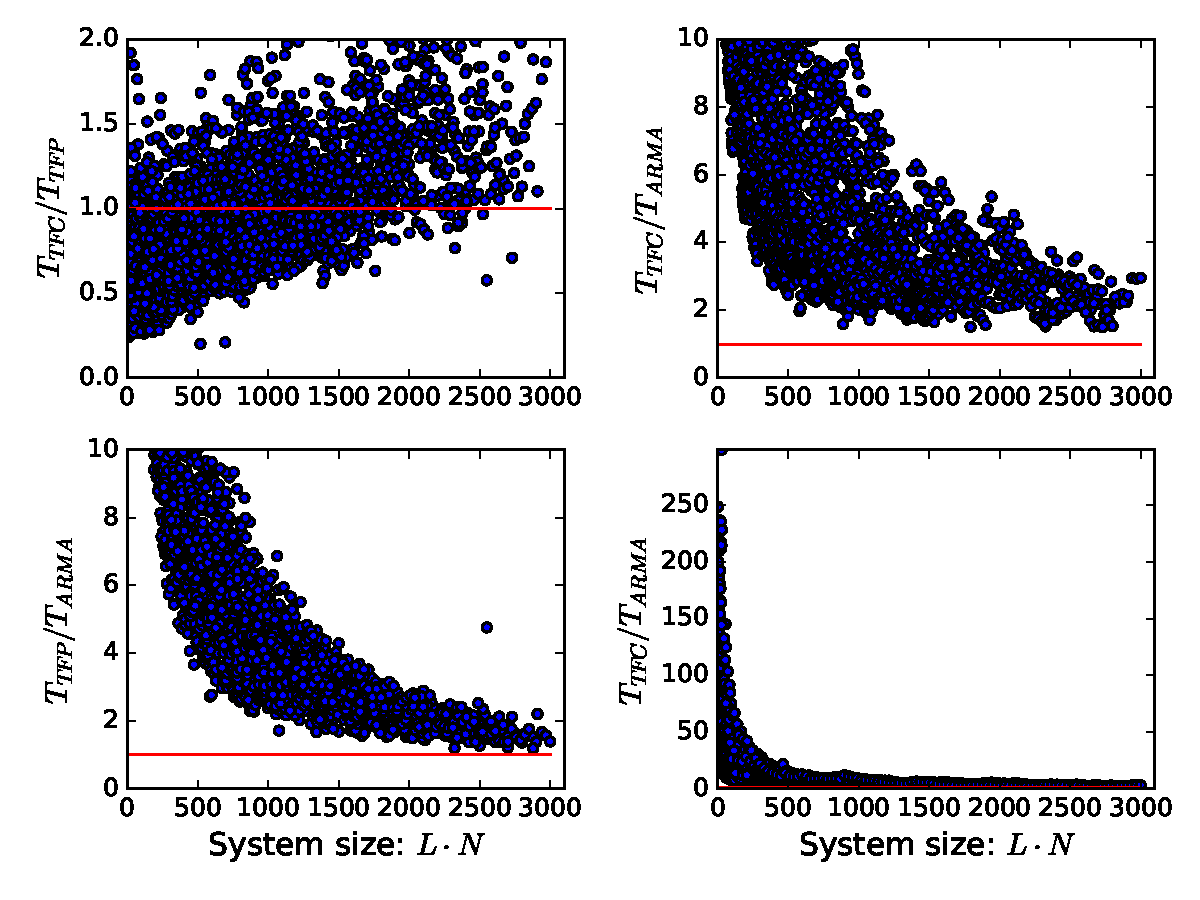
\includegraphics[width = 0.9\linewidth]{Figures/Tests/timeComparisonNetworkTotalScatter.pdf}
  \caption{Scatter plot of CPU time when evaluating untrained NNs with random weights and sigmoid activation functions
	   using the TF Python API ($T_{TFP}$), the TF C++ API ($T_{TFC}$) and Armadillo ($T_{ARMA}$). 
	   $L$ is the number of layers, $N$ is the number of nodes in each hidden layer. All the NNs
	   have one input and one output. The time has been found by averaging over 50 evaluations
	   for each NN architecture. $T_{TFC}/T_{ARMA}$ is also shown in an uncut version to demonstrate
	   how large the time difference is for very small NNs.}
\label{fig:timeComparisonEvaluateNetworkTotalScatter}
\end{figure}
\begin{figure}[H]
\centering
  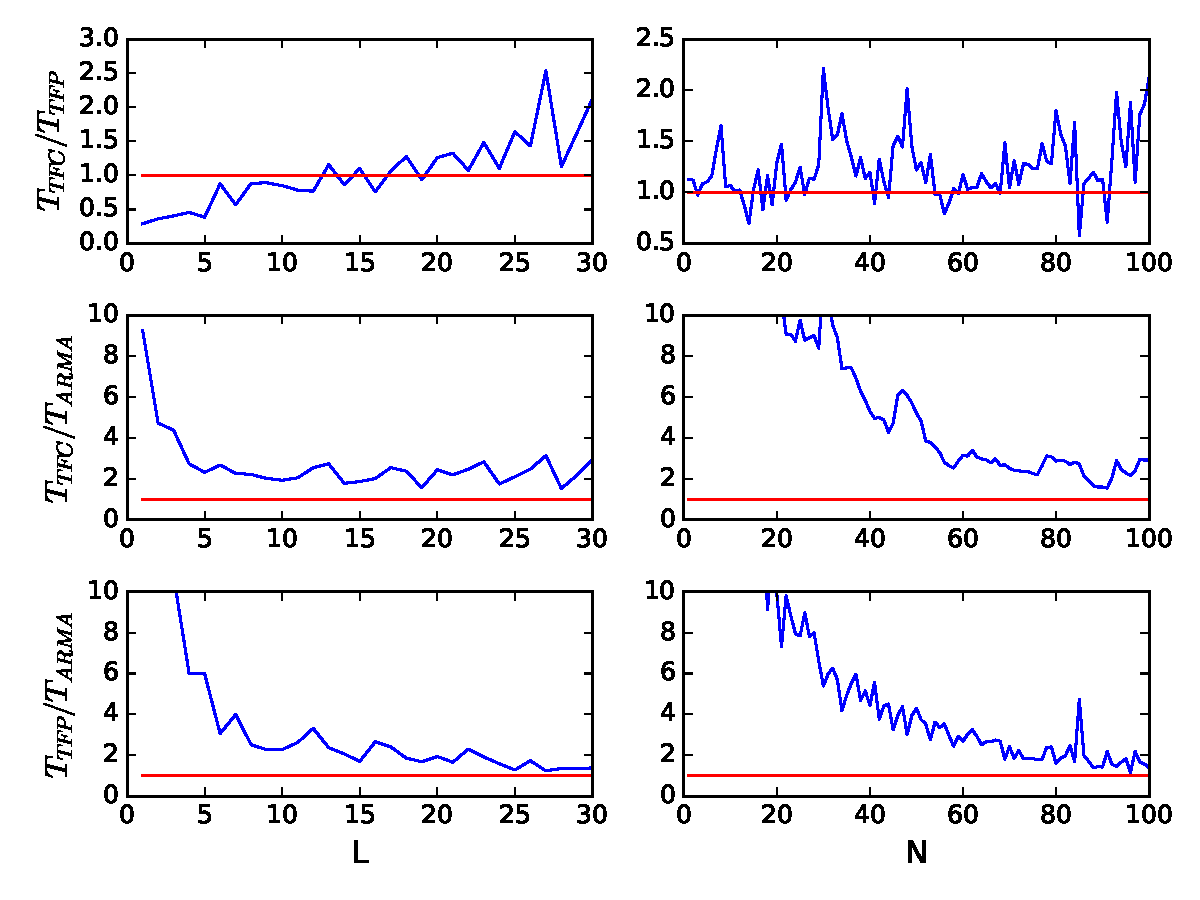
\includegraphics[width = 0.9\linewidth]{Figures/Tests/timeComparisonNetwork3.pdf}
  \caption{Left column: CPU time comparison for $N=100$. Right column: CPU time comparison for $L=30$.} 
  \label{fig:timeComparisonEvaluateNetwork2}
\end{figure}
As we can see, evaluation of an NN with the built-in TF methods are notably slower than with Armadillo 
for small NNs, but seems to converge to 1 for large networks. The convergence rate is however surpisingly low. One reason for this
can be that the \textit{Session} environment in TF has lot of overhead. However, the main computational strength of TF resides 
in GPUs, which will be tested out later on. 


\section{Training Lennard-Jones potential}
To verify that the implementation of the NN and the backpropagation algorithm with Armadillo in our MD code is correct, 
we train a NN to reproduce the shifted Lennard Jones potential (REF TIL LIKNING). 
The error of the trained network on the training data interval is evaluated both in Python and C++. The two error
plots are shown in \autoref{fig:errorLJTest}. 
\begin{figure}[H]
\begin{minipage}[t]{0.48\linewidth}
  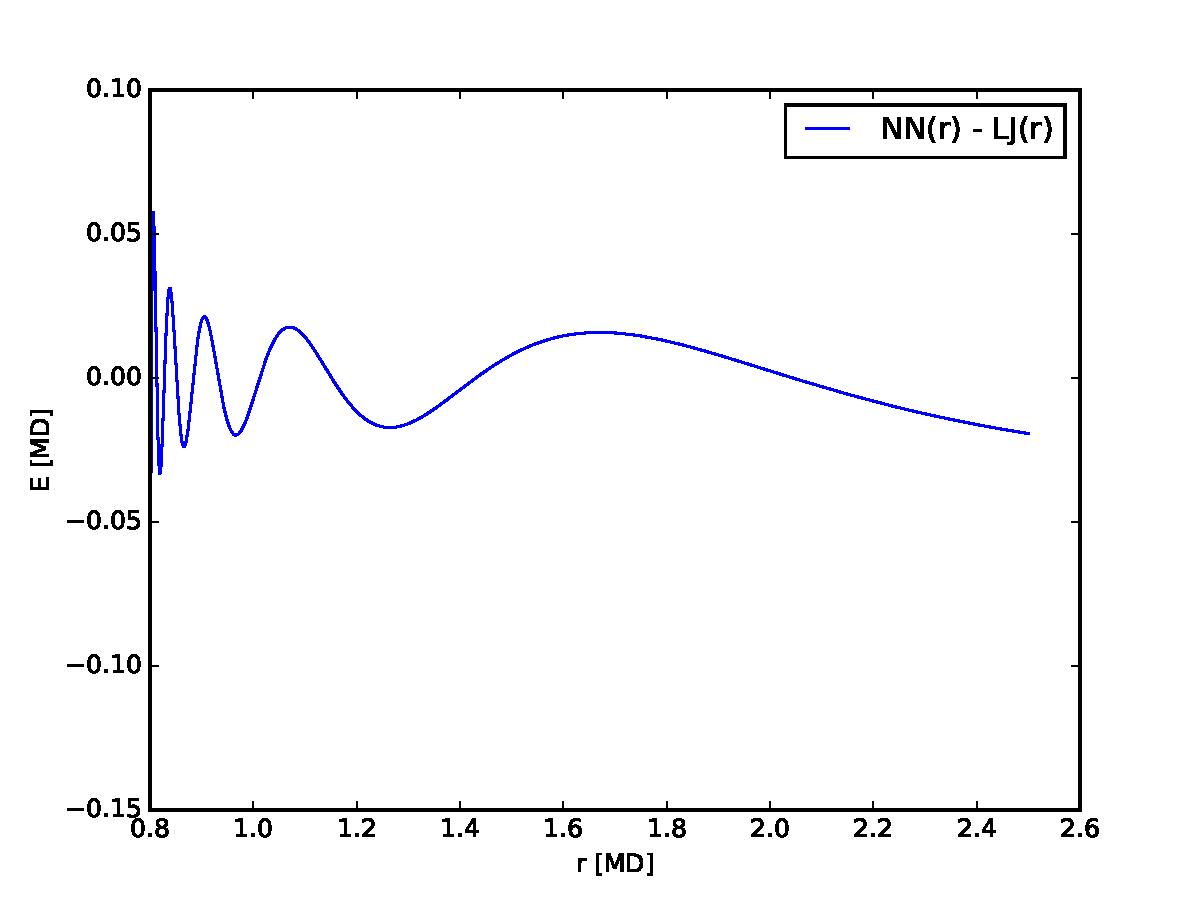
\includegraphics[width=\textwidth]{Figures/Tests/errorLJ.pdf}
\end{minipage}
\quad
\begin{minipage}[t]{0.48\linewidth}
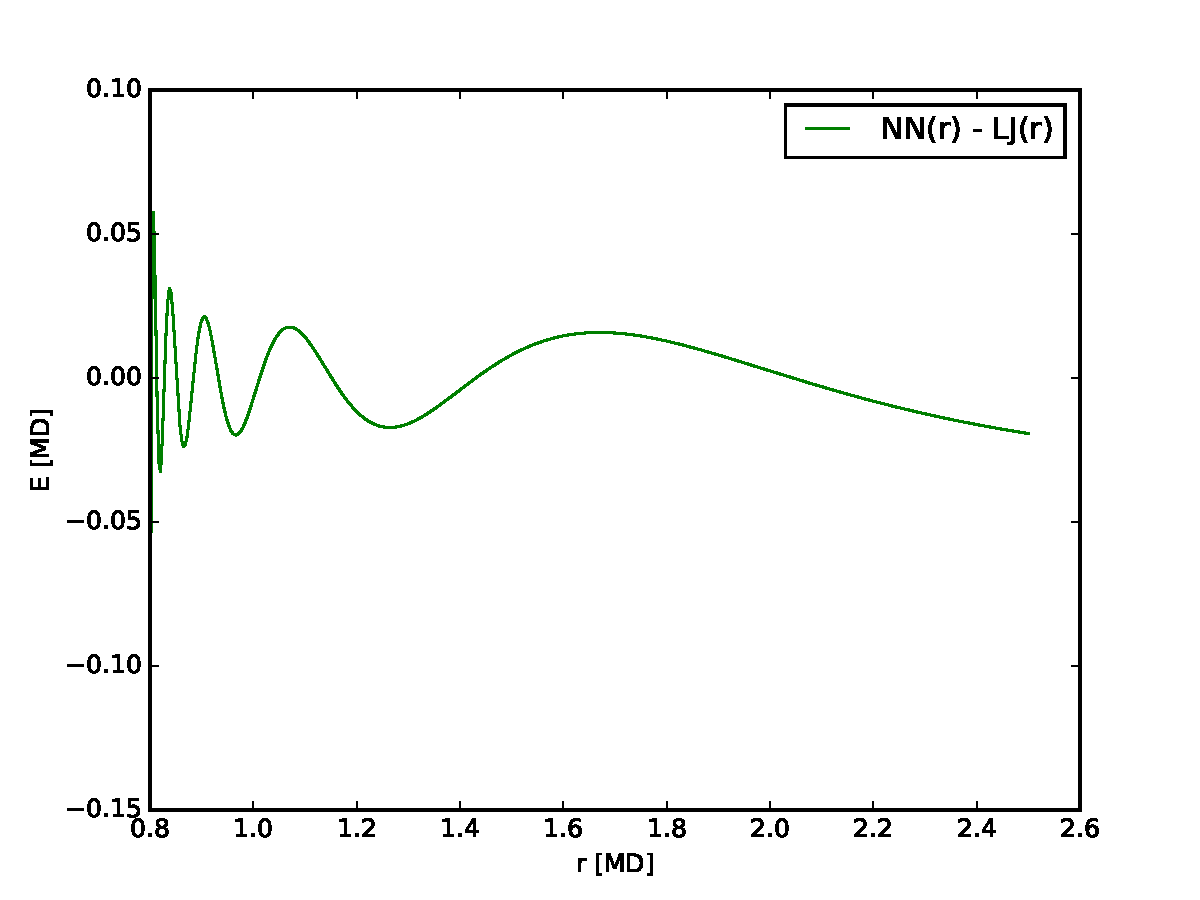
\includegraphics[width=\textwidth]{Figures/Tests/errorLJC.pdf}
\end{minipage}
  \caption{Error of a network trained to reproduce the shifted Lennard-Jones potential. 
           The NN is trained in Python and the error on the training data interval
           is calculated, shown on the left. The NN is also written to file for evaluation in C++, 
           shown on the right.}
\label{fig:errorLJTest}
\end{figure}
We observe that the error has excactly the same shape and value on the whole interval, we can therefore
confirm that the NN is implemented correctly. 

To test the implementation of the backpropagation algorithm, the
same NN is differentiated in C++ and compared to the analytical derivative of the L-J potential. 
The gradient of a NN is defined as the derivative of one of the outputs with respect to the input(s). 
There are two differences when using backpropagation to find the gradient of a network compared
to the use of backpropagation in training:
\begin{enumerate}
 \item The derivative of the output neuron's activation function is backpropagated instead of the output error
 \item We backpropagate all the way down to the input layer, during training we stop at the first hidden layer
\end{enumerate}
As mentioned before, the backpropagation algorithm is simply an application of the chain rule: 
To obtain the derivative of the output node with respect to the input nodes we need to differentiate through
all the nodes in-between because we have fully connected layers. The gradient error is plotted in 
\autoref{fig:errorBackPropTest}.
\begin{figure}[H]
\centering
  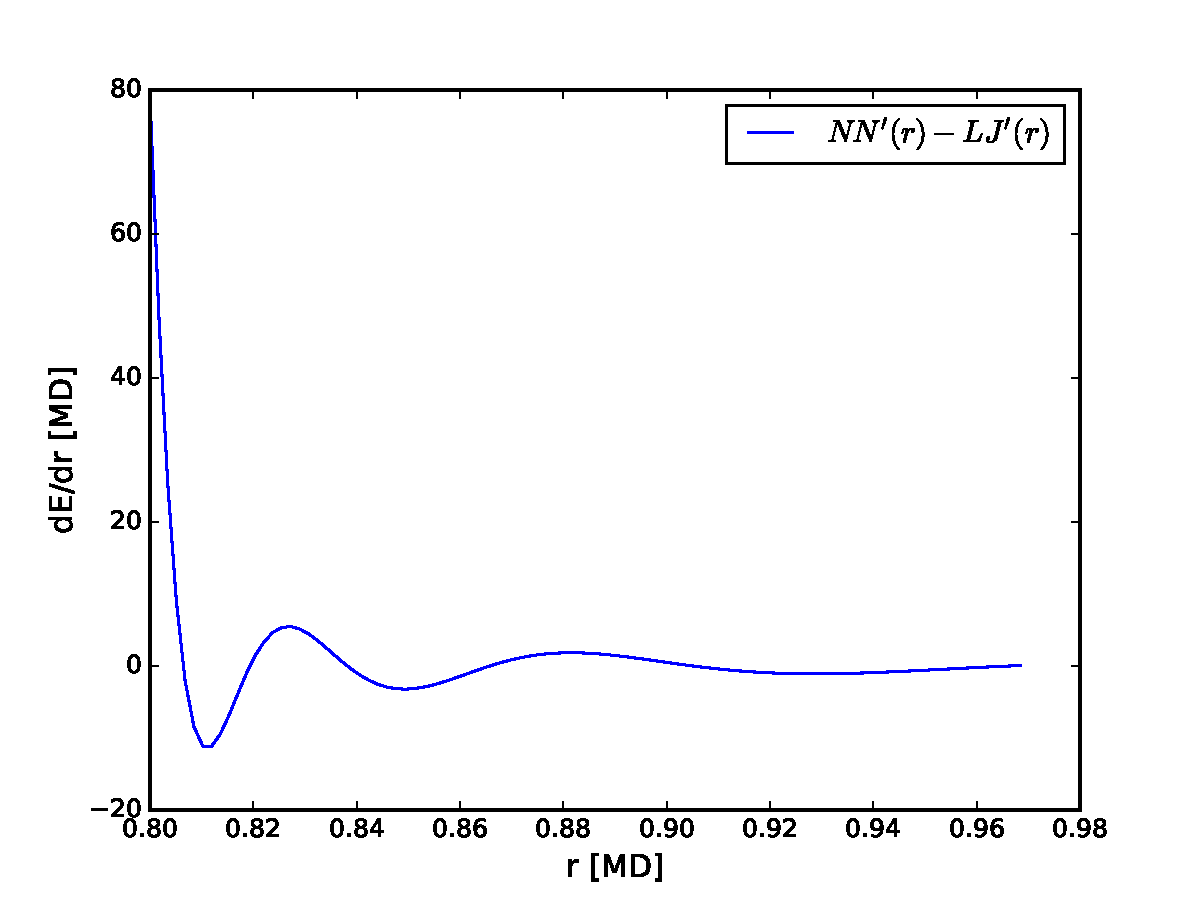
\includegraphics[width = 0.9\linewidth]{Figures/Tests/errorDerivative.pdf}
  \caption{Error of the gradient of a NN trained to reproduce the shifted Lennard-Jones potential.
	   The NN is trained in Python and evaluated and differentiated in C++ using the backpropagation algorithm.
	   The result is compared to the analytical derivative of the LJ potential. Only a part of the training
	   interval is shown, the graph is essentially flat after this point} 
  \label{fig:errorBackPropTest}
\end{figure}
Again we get an oscillating error over the training interval. The oscillations near the left end of the interval is much larger
than for the energy, but they get damped more quickly. The large error near the left end of the interval is a natural
consequence of the shape of the LJ potential for these values: the $1/r^{13}$ term dominates with its very steep slope, the NN is not 
fed a sufficient amount of data in this region to excactly reproduce the rapid changing derivative. 
This tells us that it is important to train the NN on a larger data interval than needed in simulations or possibly
feed the NN more data in critical regions during training. 

\subsection{Many-neighbour Lennard-Jones}
A NN can also be trained to obtain the energy of several neighbouring atoms at once. 
The training procedure is excactly the same, but now we train the network so that the output
is the sum of $N$ LJ-potentials for $N$ different distances $r$. The NN will have $N$ inputs and 1 output. 
To get an error of the same order as for 1 neighbour, we need to have a lot more nodes. The result of a training
session with $N=20$ inputs is shown in figures \autoref{fig:trainingManyNeighbourNN}. 
(Training session 02.12-19.36.50)
\begin{comment}
\begin{figure}[H]
\centering
  \begin{subfigure}[b]{0.75\textwidth}
  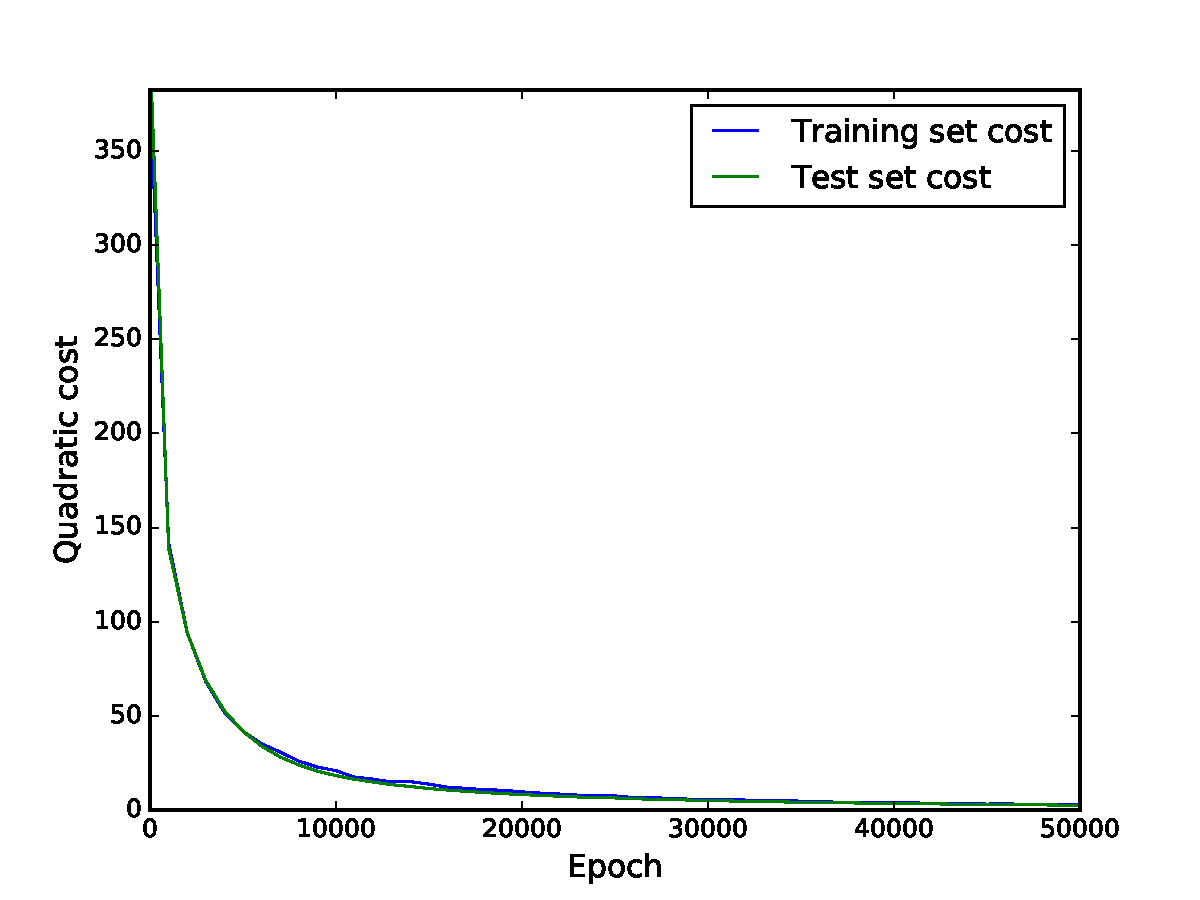
\includegraphics[width = 0.9\linewidth]{Figures/Tests/trainingManyNeighbourNN1.pdf}
\end{subfigure}
\begin{subfigure}
  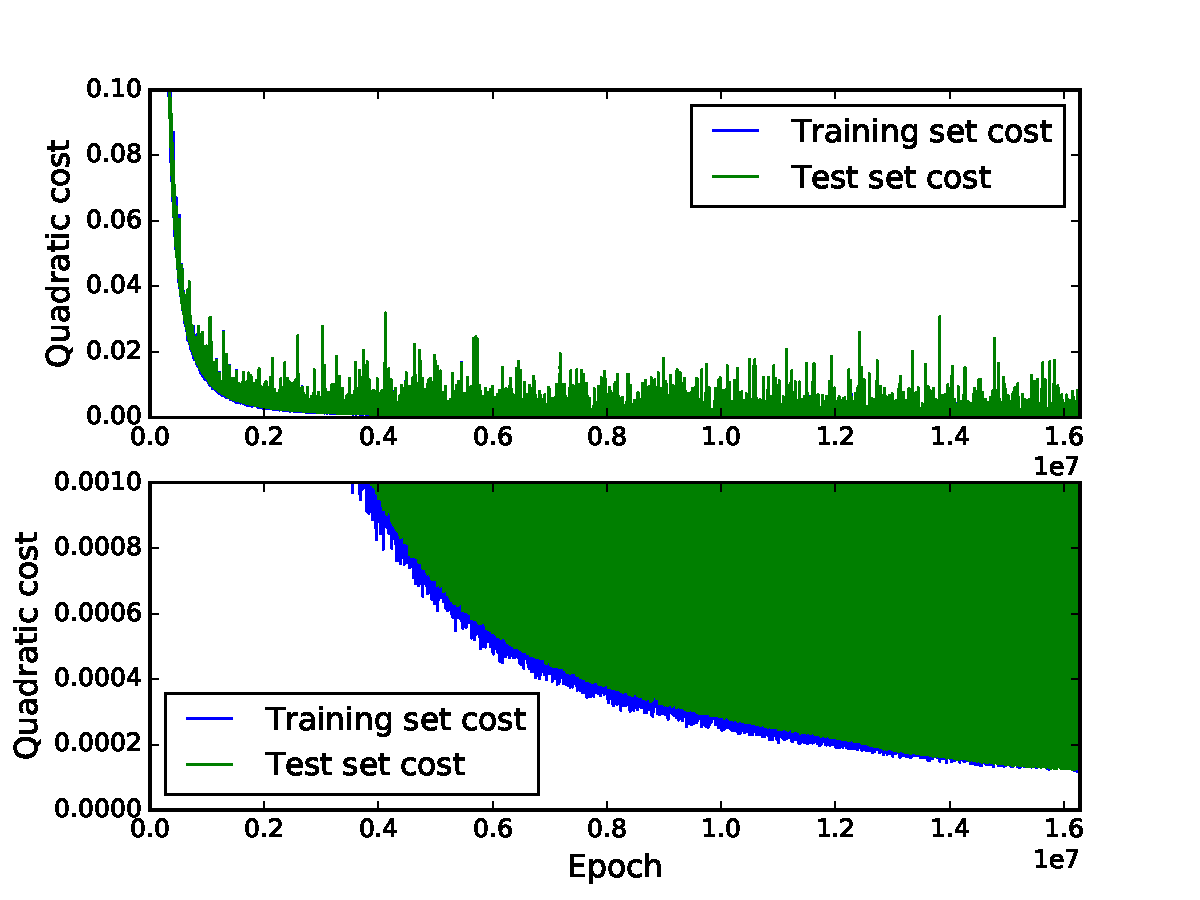
\includegraphics[width = 0.9\linewidth]{Figures/Tests/trainingManyNeighbourNN2.pdf}
  \end{subfigure}
  \label{fig:trainingManyNeighbourNN1}
  \caption{Error of the gradient of a NN trained to reproduce the shifted Lennard-Jones potential.
	   The NN is trained in Python and evaluated and differentiated in C++ using the backpropagation algorithm.
	   The result is compared to the analytical derivative of the LJ potential. Only a part of the training
	   interval is shown, the graph is essentially flat after this point} 
\end{figure}
\end{comment}
\begin{figure}[H]
\centering
\subcaptionbox{Zoomed out\label{zoomedOut}}{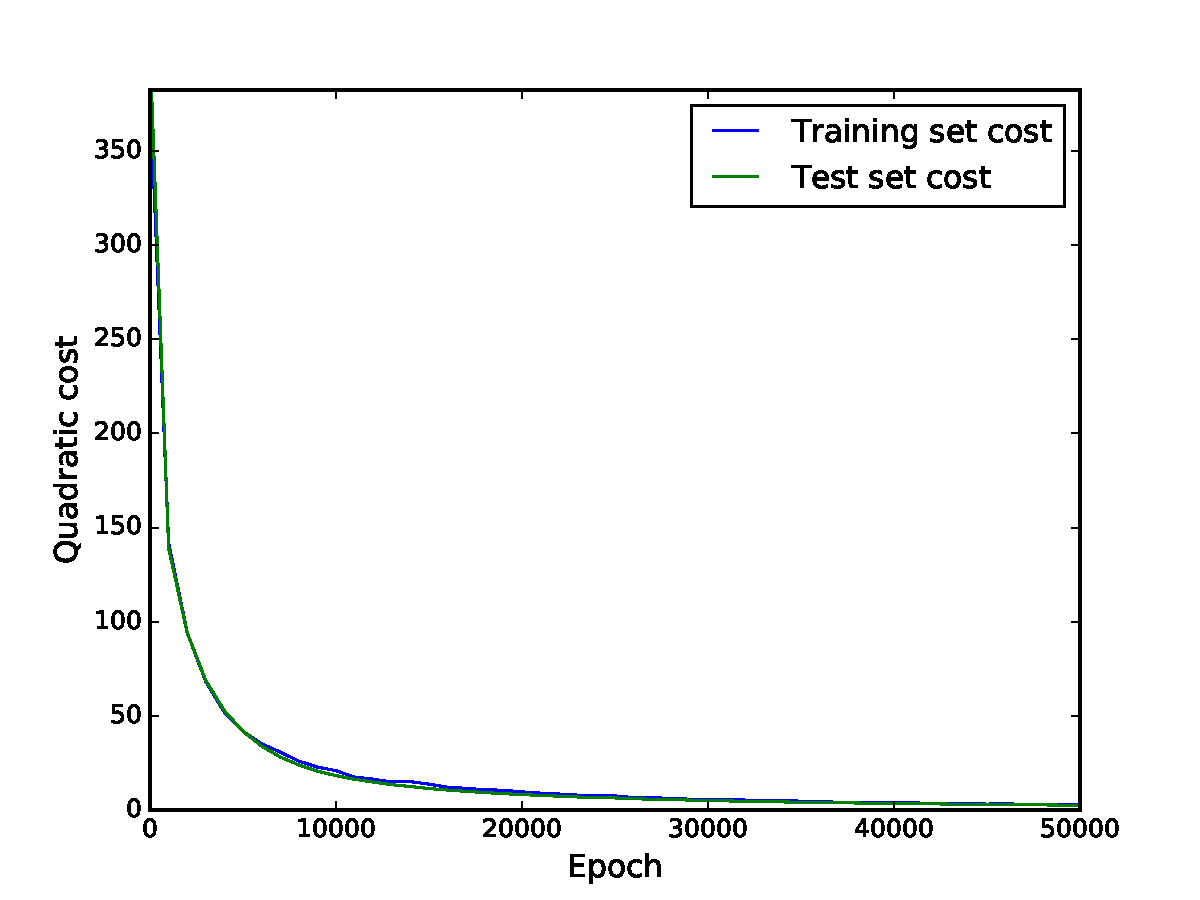
\includegraphics[width=0.8\textwidth]{Figures/Tests/trainingManyNeighbourNN1.pdf}
  }
\subcaptionbox{Zoomed in\label{zoomedIn}}{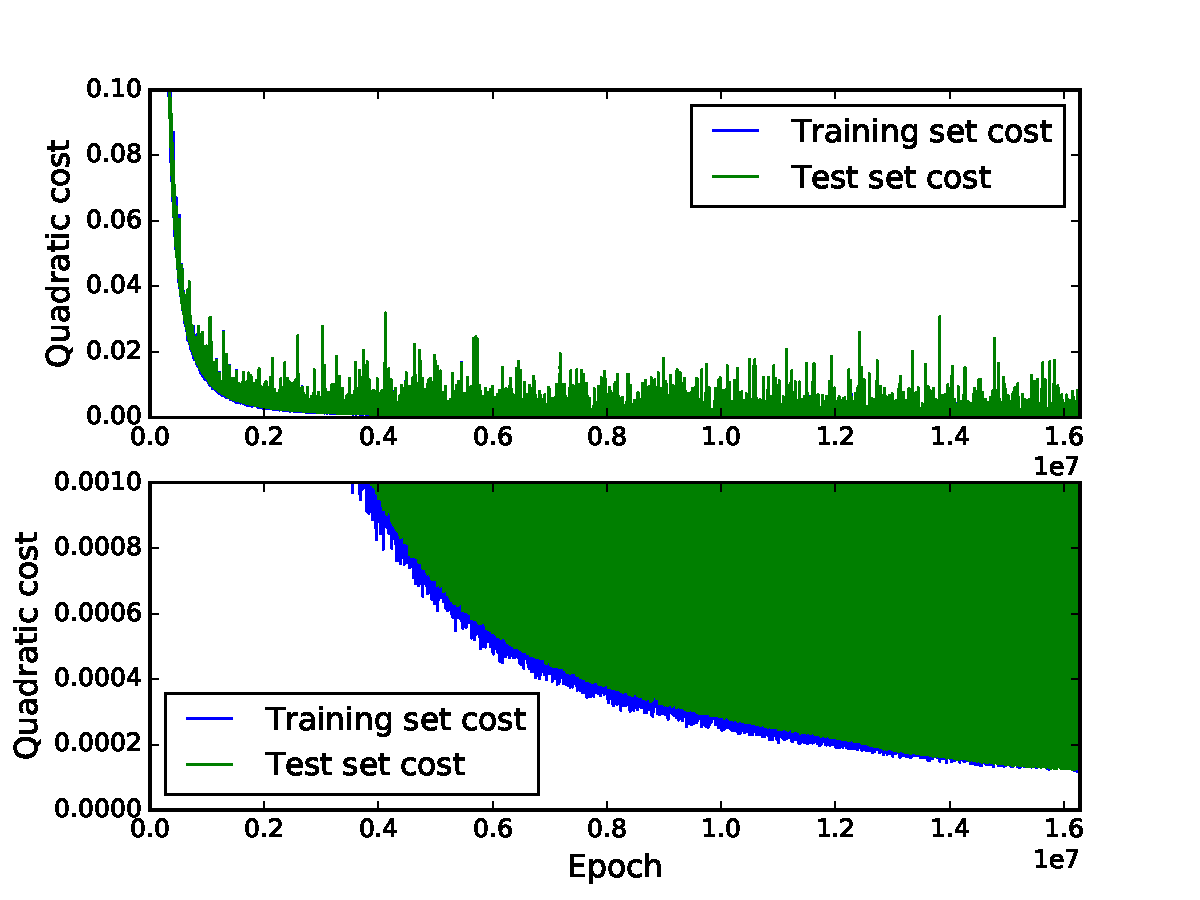
\includegraphics[width=0.8\textwidth]{Figures/Tests/trainingManyNeighbourNN2.pdf}}
\caption{Quadratic cost \eqref{quadraticCostFunction} of training set and test set for NN trained to yield
	 the sum of the shifted LJ-potential of 20 neighbouring atoms. 
	 The NN has 20 inputs, one hidden layer 
	 with 200 neurons and one output node. All nodes in the hidden layer have sigmoid activation functions 
	 \eqref{sigmoidActivationFunction}. \autoref{zoomedOut} shows the cost for the first 50 000 epochs, while
	 \autoref{zoomedIn} displays the cost for all epochs, but on a smaller scale.}	 
\label{fig:trainingManyNeighbourNN}
\end{figure}
The cost rapidly decreases during the first 10 000 epochs, then it starts to flatten out. This behaviour seems
to be general when doing regression with ANNs. 
There is no sign of overfitting: we do not observe an increase in the test cost relative to the training cost. 
This is (PROBABLY) due to the fact that our training set and test set are random numbers, i.e. there will be no 
specifics patterns or configurations present in the test set that is not covered by the training set. 
When we start doing training on data produced by MD trajectories or QM calculations, the situation will different.

The NN above outputs the total energy on an atom that is surrounded by $N$ neighbouring atoms, but it does not provide the forces. 
These must be obtained by calculating the analytical derivative of the NN with backpropagation as described above for each time step.
An alternative approach that may speed up the MD simulation is to have the NN also output the total force on the central atom. 
This can be done giving the cartesian coordinates and distance of N atoms as input to the NN so that each input
vector looks like
\begin{equation}
 (x_1, y_1, z_1, r_1, x_2, y_2, z_2, r_2, \dots, x_N, y_N, z_N, r_N)
\end{equation}
which yields an output vector
\begin{equation}
 (F_x^{TOT}, F_y^{TOT}, F_z^{TOT}, E^{TOT})
\end{equation}
We have to make sure that the input coordinates are in the range 
$x, y, z \in [-r_{cut}, r_{cut}]$ to cover the whole configuration space. The distances however, are still in the range
$r \in [a, r_{cut}]$ where $a$ is the minimum distance that two atoms can have in a given MD simulation (see function
\textit{energyAndForceCoordinates} in \textit{generateData}). As the NN now have 4 inputs per neighbour and 4 outputs, 
we need to have more nodes to get a sufficiently low error. We run a training session with 5 neighbours (20 inputs) 
(session 13.12-12.59.51). The cost has the same shape as before, but the error is much larger to begin with and also converges
slower (SKAL JEG GIDDE Å HA ENDA ET ERROR PLOT HER?).

One way to test if this works is to move only one of the input atoms while freezing the others and see if we reproduce
the LJ-potential form. We load the above training session and test with the command 
python approximateFunction2.py --load TrainingData/13.12-12.59.51/Checkpoints/ckpt-999 --test with this code: 
\begin{lstlisting}
if testFlag:
  
  # pick an input vector
  coordinates = xTrain[0]
  coordinates = coordinates.reshape([1,self.inputs])
  neighbours = self.inputs/4
  xNN = np.zeros(neighbours)
  yNN = np.zeros(neighbours)
  zNN = np.zeros(neighbours)
  rNN = np.zeros(neighbours)
  # extract coordinates and distances
  for i in range(neighbours):
      xNN[i] = coordinates[0,i*4]
      yNN[i] = coordinates[0,i*4 + 1]
      zNN[i] = coordinates[0,i*4 + 2]
      rNN[i] = coordinates[0,i*4 + 3]
		  
  # vary coordinates of only one atom and see 
  # if the resulting potential is similar to LJ
  N = 500
  r = np.linspace(0.8, 2.5, N)
  energyNN = []
  energyLJ = []
  forceNN = []
  forceLJ = []
  xyz = np.zeros(3)
  for i in range(N):
      r2 = r[i]**2
      xyz[0] = np.random.uniform(0, r2)
      xyz[1] = np.random.uniform(0, r2-xyz[0])
      xyz[2] = r2 - xyz[0] - xyz[1]
      #np.random.shuffle(xyz)
      x = np.sqrt(xyz[0])# * np.random.choice([-1,1])
      y = np.sqrt(xyz[1])# * np.random.choice([-1,1])
      z = np.sqrt(xyz[2])# * np.random.choice([-1,1])                      
      coordinates[0][0] = x; coordinates[0][1] = y; coordinates[0][2] = z
      coordinates[0][3] = r[i]
      energyAndForce = sess.run(prediction, feed_dict={self.x: coordinates})
      energyNN.append(energyAndForce[0][3]) 
      rNN[0] = r[i]
      energyLJ.append(np.sum(self.function(rNN)))
      forceNN.append(energyAndForce[0][0])
      xNN[0] = x
      forceLJ.append(np.sum(self.functionDerivative(rNN)*xNN/rNN))
  
  # convert to arrays
  energyNN = np.array(energyNN); energyLJ = np.array(energyLJ)
  forceNN = np.array(forceNN); forceLJ = np.array(forceLJ)
  
  # plot error 
  plt.plot(r, energyNN - energyLJ)
  plt.show()
  plt.plot(r, forceNN - forceLJ)
  plt.show()
  print 'Cost: ', (np.sum((energyNN - energyLJ)**2 + (forceNN - forceLJ)**2))/N
  
  # see if the energy is zero when all neighbours is at cutoff distance
  inputz = np.array([1.87, 1.32, 1.006, 2.5]*neighbours).reshape([1,self.inputs])
  r = np.array([2.5]*neighbours)
  energyLJ = sum(self.function(r))               
  ef = sess.run(prediction, feed_dict={self.x: inputz})
  
  print 'Approximate energy: ', ef[0,3]
  print 'LJ energy: ', energyLJ
  
  numberOfEpochs = 0
\end{lstlisting}
which produces the following output: 
\begin{lstlisting}
Model restored
Cost:  0.132622806039
NN energy at cutoff:  0.125104
LJ energy at cutoff:  0.0
Time elapsed: 1.2e-05
\end{lstlisting}
We see that the NN energy at cutoff is not zero, because of the cost (IS THIS CORRECT? THE COST AT CUTOFF IS PRACTICALLY ZERO).
The error of the NN energy and forces over the training data interval is shown in 
\begin{figure}[H]
\begin{minipage}[t]{0.48\linewidth}
  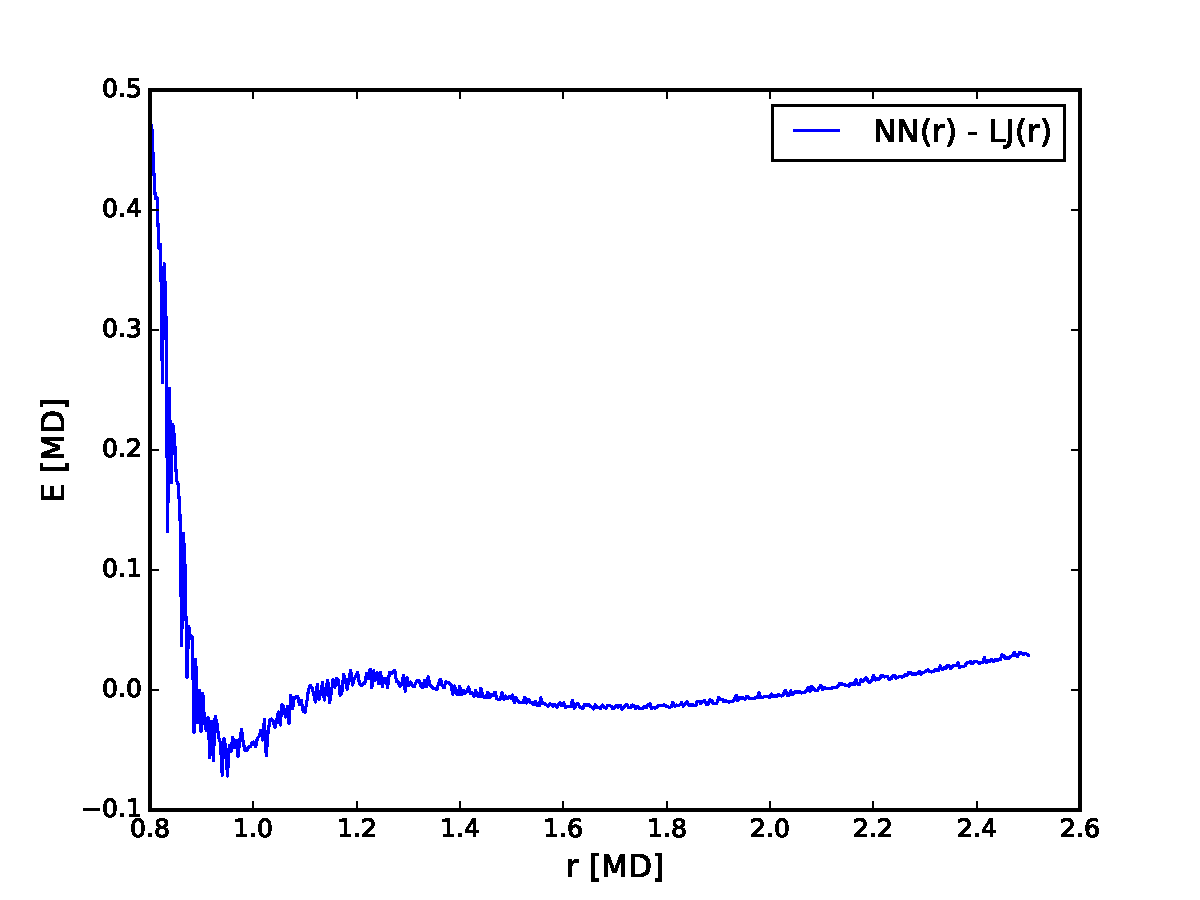
\includegraphics[width=\textwidth]{Figures/Tests/manyNeighbourEnergyError.pdf}
\end{minipage}
\quad
\begin{minipage}[t]{0.48\linewidth}
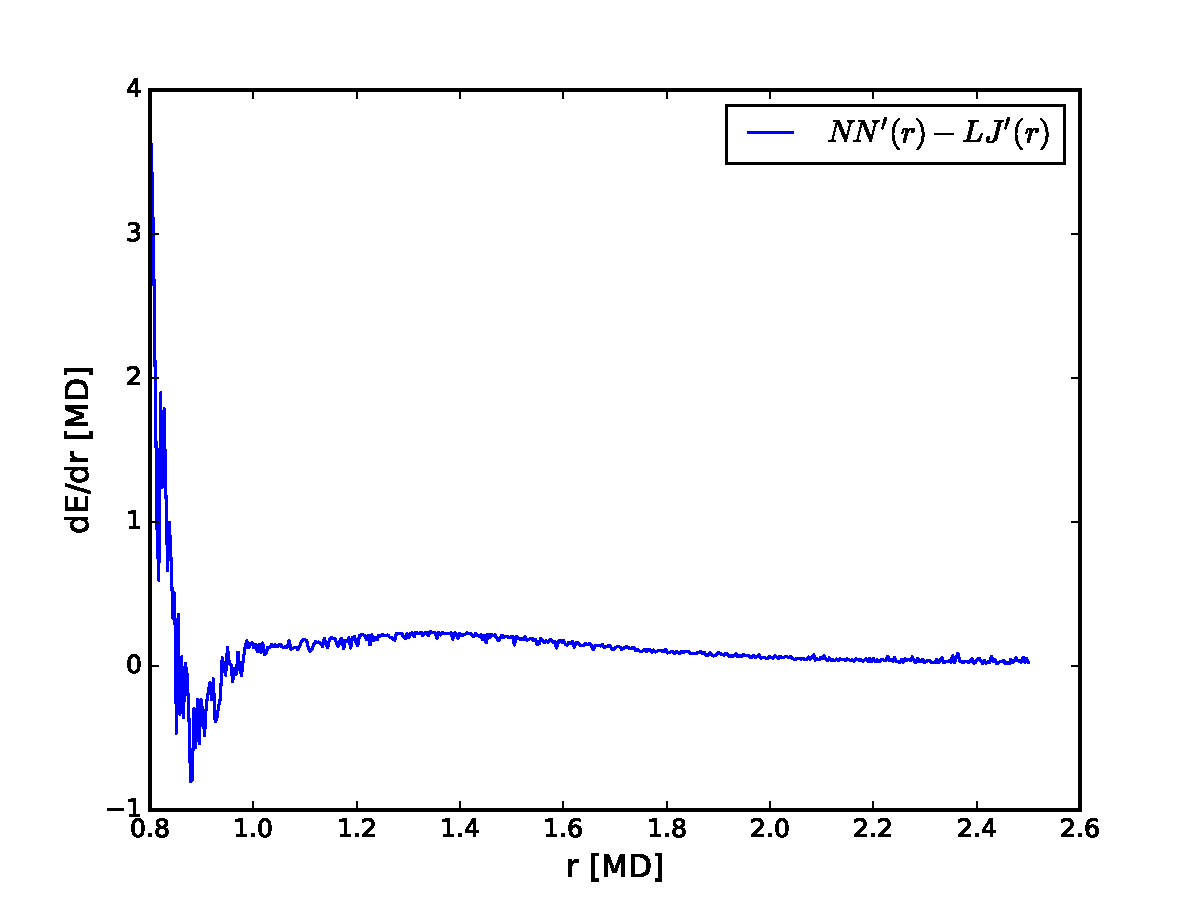
\includegraphics[width=\textwidth]{Figures/Tests/manyNeighbourForceError.pdf}
\end{minipage}
  \caption{Error of a network trained to yield the total energy and force on a central atom from 5 neighbouring atoms. 
           The energy contribution from each neighbour is a shifted LJ potential. Trained for 1e6 epochs, 100 nodes
           in 2 layers. The energy error is shown on the left, force error on the right.}
\label{fig:errorManyNeighbourNN}
\end{figure}
The error oscillates in exactly the same way as for the 1-input NN above, suggesting that the training is done correctly. 
However, it is very important that the energies and forces in an MD simulation is consistent, and this is not 
ensured here, where the two are obtained in a somewhat independent way. Any incosistency between the energies and forces
will magnify for each time step, resulting in inaccurate statistical properties like temperature and pressure. 
Therefore it is a better idea to have the NN only output the total energy, and find the forces by analytically
differentiating the NN for each time step. $\SI{4}{\angstrom}$


\newpage 
%\section{Appendix}
\appendix
\section{Appendix}
\subsection{Symmetry functions derivatives} \label{app:appendixA1}
We list here the derivatives of the symmetry functions used for training neural networks. These have to be known
to compute forces for MD simulations. In some cases we only show the deriviative with respect to 
$R = \sqrt{x^2 + y^2 + z^2}$. 
Each component $\alpha$ can be calculated by
\begin{equation}
 \frac{\partial R}{\partial \alpha} = \frac{\alpha}{R}
\end{equation}
Cutoff function \eqref{cutoffFunction}:
\begin{equation}
 \frac{\partial f_c(R)}{\partial R} = -\frac{1}{2}\frac{\pi}{R_c} \sin\left(\frac{\pi R}{R_c}\right) = M(R)
 \label{cutOffFunctionDerivative}
\end{equation}
This expression is valid for all combinations of indicies. The derivatives w.r.t. to individual coordinates are
\begin{equation}
 \frac{\partial f_c(R_{ij})}{\partial x_{ij}} = M(R_{ij})
 \frac{x_{ij}}{R_{ij}}
 \label{cutOffFunctionDerivative1}
\end{equation}
and 
\begin{equation}
 \frac{\partial f_c(R_{ik})}{\partial x_{ik}} = M(R_{ik})
 \frac{x_{ik}}{R_{ik}}
 \label{cutOffFunctionDerivative1}
\end{equation}
while
\begin{equation}
 \frac{\partial f_c(R_{ij})}{\partial x_{ik}} = \frac{\partial f_c(R_{ik})}{\partial x_{ij}} = 0
\end{equation}
because atom $i$ is always in origo, which means we can do the substitutions $x_{ij} \rightarrow x_{j}$ and 
$x_{ik} \rightarrow x_{k}$. SHOULD I DO THIS CONSEQUENTLY BELOW????. Also, 
\begin{equation}
 \frac{\partial f_c(R_{jk})}{\partial x_{ij}} = M(R_{jk})
 \frac{x_{jk}}{R_{jk}}
 \label{cutOffFunctionDerivative1}
\end{equation}
and 
\begin{equation}
 \frac{\partial f_c(R_{jk})}{\partial x_{ij}} = -M(R_{jk})
 \frac{x_{jk}}{R_{jk}}
 \label{cutOffFunctionDerivative1}
\end{equation}
The derivative of each term in $G_i^1$ \eqref{G1} is simply \eqref{cutOffFunctionDerivative}. \\
$G_i^2$ \eqref{G2}:
\begin{equation}
 \frac{\partial G_i^2}{R_{ij}} = 
 \exp(-\eta(R_{ij}-R_s)^2) \left[2\eta(R_s - R_{ij}) + \frac{\partial f_c}{\partial R_{ij}}\right]
\end{equation}
$G_i^3$ has not been used in this theses. \\
$G_i^4$ \eqref{G4}:
\begin{equation}
 G_i^4 = 2^{1-\zeta}F_1(\theta)F_2(R_{ij},R_{ik},R_{jk})F_3(R_{ij},R_{ij},R_{jk})
\end{equation}
where
\begin{align}
 F_1(\theta) &= (1 + \lambda \cos\theta_{ijk})^\zeta \\
 F_2(R_{ij},R_{ik},R_{jk}) &= \exp[-\eta (R_{ij}^2 + R_{ik}^2 + R_{jk}^2)] \\
 F_3(R_{ij},R_{ij},R_{jk}) &= f_c(R_{ij}) f_c(R_{ik}) f_c (R_{jk})
\end{align}
where
\begin{equation}
 \cos\theta = \frac{x_{ij}x_{ik} + y_{ij}y_{ik} + z_{ij}z_{ik}}{R_{ij}R_{ik}}
\end{equation}
Using the product rule:
\begin{align}
 \frac{\partial G_i^4}{\partial x_{ij}} = &\frac{\partial F_1}{x_{ij}} F_2 F_3 + 
 F_1 \left(\frac{\partial F_2}{\partial x_{ij}}F_3 + F_2\frac{\partial F_3}{\partial x_{ij}}\right) \\
 &\frac{\partial F_1}{x_{ij}} F_2 F_3 + 
 F_1 \frac{\partial F_2}{\partial x_{ij}}F_3 + F_1F_2\frac{\partial F_3}{\partial x_{ij}}
 \label{G4Derivative}
\end{align}
We have
\begin{equation}
 \frac{\partial F_1}{\partial x_{ij}} = \frac{\partial F_1}{\partial\cos\theta}
 \frac{\partial\cos\theta}{\partial x_{ij}}
\end{equation}
where
\begin{equation}
 \frac{\partial F_1}{\partial\cos\theta} = \lambda\zeta(1 + \cos\theta)^{\zeta-1} = K
\end{equation}
and 
\begin{equation}
 \frac{\partial\cos\theta}{\partial x_{ij}} = \frac{x_{ik}}{r_{ij}r_{ik}} - 
 \frac{x_{ij}\cos\theta}{r_{ij}^2}
\end{equation}
To get the corresponding expression for $x_{ik}$, simply substitute $x_{ij} \leftrightarrow x_{ik}$ and 
$r_{ij} \leftrightarrow r_{ik}$. Further, 
\begin{align}
 \frac{\partial F_2}{\partial x_{ij}} &= \frac{\partial F_2}{\partial r_{ij}}\frac{\partial r_{ij}}{\partial x_{ij}}  = 
 -2\eta r_{ij}\exp[-\eta (R_{ij}^2 + R_{ik}^2 + R_{jk}^2)] \frac{x_{ij}}{r_{ij}} \\
 &= -2\eta \exp[-\eta (R_{ij}^2 + R_{ik}^2 + R_{jk}^2)] x_{ij} = Lx_{ij}
\end{align}
The corresponding expression for $x_{ik}$ is obtained by substituing $x_{ij} \rightarrow x_{ik}$. 
Lastly, 
\begin{align}
 \frac{\partial F_3}{\partial x_{ij}} &=  \frac{\partial f_c(r_{ij})}{\partial x_{ij}}
 f_c(r_{ik}) f_c(r_{jk}) + f_c(r_{ij})f_c(r_{ik})\frac{\partial f_c(r_{jk})}{\partial x_{ij}} \\
 &= f_c(r_{ik})\Biggr(M(r_{ij})\frac{x_{ij}}{r_{ij}}f_c(r_{jk}) + 
 f_c(r_{ij}) M(r_{jk})\frac{x_{jk}}{r_{jk}} \Biggr)
\end{align}
The corresponding expression for $x_{ik}$ is
\begin{align}
 \frac{\partial F_3}{\partial x_{ik}} &= f_c(r_{ij})\Biggr(\frac{\partial f_c(r_{ik})}{\partial x_{ik}}f_c(r_{jk}) + 
 f_c(r_{ik}) \frac{\partial f_c(r_{jk})}{\partial x_{ik}} \Biggr) \\
 &= f_c(r_{ij})\Biggr(M(r_{ik})\frac{x_{ik}}{r_{ik}}f_c(r_{jk}) - 
 f_c(r_{ik}) M(r_{jk})\frac{x_{jk}}{r_{jk}} \Biggr) \\
\end{align}

Then, taking \eqref{G4Derivative} into account:
\begin{align}
 \frac{\partial G_i^4}{\partial x_{ij}} &= \biggr(\frac{x_{ik}}{r_{ij}r_{ik}} - \frac{x_{ij}\cos\theta}{r_{ij}^2}
 \biggr)KF_2F_3 + x_{ij}F_1LF_3 \\
 &+ F_1F_2 f_c(r_{ik})\Biggr(M(r_{ij})\frac{x_{ij}}{r_{ij}}f_c(r_{jk}) + 
 f_c(r_{ij}) M(r_{jk})\frac{x_{jk}}{r_{jk}} \Biggr)
\end{align}
and for $x_{ik}$:
\begin{align}
 \frac{\partial G_i^4}{\partial x_{ik}} &= \biggr(\frac{x_{ij}}{r_{ij}r_{ik}} - \frac{x_{ik}\cos\theta}{r_{ik}^2}
 \biggr)KF_2F_3 + x_{ik}F_1LF_3 \\
 &+ F_1F_2 f_c(r_{ij})\Biggr(M(r_{ik})\frac{x_{ik}}{r_{ik}}f_c(r_{jk}) - 
 f_c(r_{ik}) M(r_{jk})\frac{x_{jk}}{r_{jk}} \Biggr)
\end{align}
or in terms of $x_{ij}$ and $x_{ik}$ and $x_{jk}$:
\begin{align}
 \frac{\partial G_i^4}{\partial x_{ij}} = &x_{ij} \biggr(-\frac{\cos\theta}{r_{ij}^2}K
 F_2F_3 + F_1LF_3 + F_1F_2M(r_{ij})f_c(r_{ik})f_c(r_{jk})\frac{1}{r_{ij}}\biggr) + \\
 &x_{ik}\frac{KF_2F_3}{r_{ij}r_{ik}} + x_{jk}F_1F_2M(r_{jk})f_c(r_{ik})f_c(r_{ij})\frac{1}{r_{jk}}
\end{align}
and 
\begin{align}
 \frac{\partial G_i^4}{\partial x_{ik}} = &x_{ik} \biggr(-\frac{\cos\theta}{r_{ik}^2}K
 F_2F_3 + F_1LF_3 + F_1F_2M(r_{ik})f_c(r_{ij})f_c(r_{jk})\frac{1}{r_{ik}}\biggr) + \\
 &x_{ij}\frac{KF_2F_3}{r_{ij}r_{ik}} - x_{jk}F_1F_2M(r_{jk})f_c(r_{ij})f_c(r_{ik})\frac{1}{r_{jk}}
\end{align}









\newpage

\begin{thebibliography}{9}

\bibitem{ref1}
 J. Behler
 \textit{Neural network potential-energy surfaces in chemistry: a tool for large-scale simulations}
 Phys. Chem. Chem. Phys., 2011, {\bf 13}, 17930-17955 (2011)
 
\bibitem{ref2}
 Dragly, Svenn Arne
 \textit{Bridging quantum mechanics and molecular dynamics with artificial neural networks}
 Thesis for the degree of Master of Science, University of Oslo (2014)

\bibitem{ref3}
 K. Hornik, M. Stinchcombe and H. White
 \textit{Multilayer Feedforward Networks are Universal Approximators}
 Neural Networks {\bf 2}, 359 (1989).
 
\bibitem{ref4}
 R. Rojas. 
 \textit{Neural Networks: A Systematic Introduction.}
 Springer, 1996.
 
\bibitem{ref5}
 B. Karlik and A. V. Olgac
 \textit{Performance Analysis of Various Activation Functions in Generalized MLP Architectures of Neural Networks.}
 IJAE {\bf 1} 111-122 (2011)
 
\bibitem{ref6}
 Y. LeCun, Y. Bengio and G. Hinton
 \textit{Deep learning}
 Nature {\bf 521}, 436-444 (2015)
 
\bibitem{ref7}
 X. Glorot, A. Bordes, Y. Bengio
 \textit{Deep Sparse Rectifier Neural Networks}
 JMLR {15}, 315-323 (2011)
 
\bibitem{ref8}
 D. E. Rumelhart, G. E. Hinton and R. J. Williams
 \textit{Learning representations by back-propagating errors}
 Nature {\bf 323}, 533-536 (1986)
 
\bibitem{ref9}
 J. Behler
 \textit{Constructing High-Dimensional Neural Network Potentials: A Tutorial Review}
 International Journal of Quantum Chemistry {\bf 115}, 1032-1050 (2015)
 
\bibitem{ref10}
 J. Behler
 \textit{Neural network potential-energy surfaces in chemistry: a tool for large-scale simulations}
 Phys. Chem. Chem. Phys. {\bf 13}, 17930–17955 (2011)
 
\bibitem{ref11}
 Tuckerman, Berne and Martyna 
 \textit{Reversible multiscale molecular dynamics}
 J. Chem Phys, {\bf 97}, 1990 (1992).
 

\end{thebibliography}

\end{document}